% !TEX encoding = UTF-8 Unicode
\documentclass[draft]{article}
\usepackage{geoA4}
\usepackage{libertine}

\usepackage{els}
\usepackage{i}
\usepackage{notate}
\usepackage{wrapfig}
\newcommand{\ap}{\ensuremath{\tau}\xspace}
\newcommand{\dap}{\ensuremath{d\ap}\xspace}
%\usepackage{geoA4}
\renewcommand{\oe}{;~o.e.{}}
\renewcommand{\me}{;~m.e.{}}
\newcommand{\oemph}[1]{\emph{#1}}
\newcommand{\memph}[1]{\emph{#1}}
\newcommand{\phin}{\ensuremath{\varphi_\nu}\xspace}
\newcommand{\Lag}{\ensuremath{\mathcal{H}}\xspace}
\newcommand{\manu}[1]{\citep[#1]{Reichenbach1928b}}
\newcommand{\nbein}{$n$-bein\xspace}
\newcommand{\vbein}{vierbein\xspace}
\renewcommand{\fmn}{\ensuremath{F\mn}\xspace}
\newcommand{\hbein}{\ensuremath{h_{a}^{\nu}}\xspace}
\newcommand{\xdx}{\ensuremath{x_\nu} and \ensuremath{x_\nu + dx_\nu}\xspace}
\newcommand{\hbeinr}{\ensuremath{h_{\alpha}^{\nu}}\xspace}
\newcommand{\PRZL}{\citetitle{Reichenbach1928}\xspace}
\newcommand{\Reich}{Reichenbach\xspace}
\newcommand{\VZ}{\jt{Vossische Zeitung}\xspace}
\newcommand{\FP}{\german{Fernparallelismus}\xspace}
\newcommand{\DP}{distant parallelism\xspace}
\newcommand{\Gtmnbar}{\ensuremath{\bar{\Gamma}\tmn}\xspace}
%\newcommand{\fmn}{\ensuremath{f\mn}\xspace}
\newcommand{\faraday}{\ensuremath{\fmn}\xspace}

\newcommand{\WT}{Weyl's theory\xspace}

\newcommand{\rhp}[2]{(\cite[#1]{Reichenbach1920a}; tr.\ \citeyear{Reichenbach1969} #2)\xspace}
\renewcommand{\rzlp}[2]{(\cite[#1]{Reichenbach1928}; tr.\ #2)\xspace}
\renewcommand{\rzlap}[2]{(\cite[#1]{Reichenbach1928}; tr.\ [#2])\xspace}
\newcommand{\vza}[1]{(\cite{Reichenbach1929c}; tr.\ \citeyear{Reichenbach1978}, 1:#1)\xspace}
\newcommand{\hpa}[2]{(\cite[#1]{Reichenbach1929}; tr.\ \citeyear{Reichenbach1978}, 1:#2)\xspace}



\makeatletter
\def\tagform@#1{\maketag@@@{[\ignorespaces#1\unskip\@@italiccorr]}}
\makeatother


\creflabelformat{equation}{#2[\textup{#1}]#3}

\newlist{W}{enumerate}{1}
\setlist[W]{label=W-\Roman*}

%\usepackage{tuftefont}

%\newmdenv[linecolor=black]{infobox}
%%\renewcommand*{\multicitedelim}{\addcomma\space}
%\renewcommand*{\multicitedelim}{\addsemicolon\space}
\title{Coordination, Geometrization, Unification. An Overview of the Reichenbach--Einstein Debate on the Unified Field Theory Program}

%TODO check translaton of Reichenbach!!!
%TODO check **

\begin{document}
\maketitle

\begin{abstract}
\lipsum*[1-2]
\end{abstract}


\begin{keywords}
Reichenbach \sep Einstein \sep Weyl \sep Unified Field Theory \sep General Relativity \sep Geometrization \sep Unification \sep Coordination	
\end{keywords}

\section*{Introduction}

%1186 of the field equations (78.3) with any given distribution of matter and energy to predict the dependence of the tensor guy on the coordinates used, and then compare the predicted values of the guy with observed values of the 9 py• Theoretically, these observed values could of course be obtained from the direct measurement of space-like and time-like intervals with the help of the

%F12). The free field theory (i.e. in the absence of matter) can be cast into Lagrangian form with L=-}F.Fap choosing as the fundamental quantities the potentials, the scalar potential  and the vector potential A. These are required to transform

%The field equations, Maxwell equations, were derived from a variational principle from single Lagrangian \Lag choosing treating the four-potential potentials \phin as independent fields\todo{check}.\footnoteh{A field theory source variables (mass density, charge density and the like) represent the sources of the field in question and field variables (gravitational field, electromagnetic field, and so on) represent the forces arising from the interaction. The theory provides field equations, which relate the source variables to the field variables, and equations of motion, which pick out a privileged class of trajectories with the help of the field variables}  In the theory of electrons it is assumed that ponderable bodies contain small positively and negatively charged particles, the term electron usually being applied to both types of charged particle. A force is exerted upon electrons by an electromagnetic field. A conductor is characterized by the

%The first successful field theory was created by Maxwell in the mid-19th century, and brought to his completion by Lorentz at the turn of the century in the form of the theory of the electron, based on the strict separation between field and matter. Ponderable bodies contain small positively and negatively charged particles, electrons, which generate electric and magnetic fields obeying Maxwell’s field equations. These charged particles in turn are acted upon by those fields according to Lorentz force law. After \citets{Einstein1905} \sr, by 1908, \citet{Minkowski19078} was able to cast Maxwell's theory in a four-dimensional form. Electric and magnetic fields strengths turned out to be components of a single electromagnetic field represented by a skew-symmetric tensor \fmn. Given a certain distribution of sources (electrons at rest and in motions) Maxwell's field equations make predictions about the distribution of \fmn at a certain points \xn with respect to an inertial frame. These predictions, in principles, could be tested empirically. The position of a point \xn with respect to an inertial frame can be measured with \rac and the values of the \fmn at that point can be determined by observing the acceleration of charge test particles according to Lorentz force law.  

%The peculiarities of the gravitational field, encoded in the equivalence principle, exposed the limitations of special relativity and ultimately burst its framework. Only a decade later, by 1915, \citet{Einstein1916} managed to formulate a field theory of gravitation that took the place of Newton's action-at-a-distance theory. The fixed structure of Minkowski's \spti had to be generalized to dynamical Riemannian metric in which the symmetric tensor \gmn plays the role of gravitational potentials and described the behave of \rac with respect to a coordinate system. Given a certain distribution of sources (matter and energy) Einstein's field equations predict the dependence of the tensor \gmn on the coordinates. Also in this case, the theory could be in principle tested empirically, since the values of \gmn with respect to a certain \cs can be measured with \rac, or indirectly by the motion of light rays and test particles\footnote{For the conceptual difficulties} following the geodesic equation.

%\footnote{The testing of \gr implies more substantive difficulties}\todo{tolman, rockets, difficulties}

%but rather as an aspect of the geometrical structure of space-time

%By the end of the 1910s, physicists could rely on two successful field theories. The relations between them, however, was rather extrinsic\todo{better}. The gravitational field \gmn occupied a privileged position with respect to the electromagnetic field. One can imagine a \spti without an electromagnetic field \fmn, but there can be no \spti without the gravitational field \gmn since the latter also incorporates the geometrical structure of \spti. The electromagnetic field \fmn and gravitational field \gmn rested upon a different and independent mathematical structures. \citep{Einstein1920}. Since the elementary particles of matter, the positive and negative electron were supposed to be nothing  but condensations of the electromagnetic field, the separation between two fields also implied the separation between field and matter as the source of the field \citep{Einstein1920}. Many felt that these dualisms were theoretically unacceptable\todo{??}. 



%Soon relativists started to search for a \scare{unified field theory} which would combine both gravitational field and electromagnetic field into a unified geometrical structure and at the same time integrate the field with its sources. The quixotic\footnote{The expression is used by Einstein himself on several occasions; see \eg \letterspeziali{Einstein}{Besso}{15}{4}{1950}[172]; \letteraea{Einstein}{Laue}{17}{1}{1951}[16-168]; \letteraea{Einstein}{Bohm}{24}{11}{1954}[8-055]; \letterund{Einstein}{Born}[\citep[\D{93}, undated]{Born1971}]} quest for the final field theory spans over 


Most of Einstein's published work from 1919 till his death in 1955 \citep{Einstein1955-07}\footnote{For an overview of Einstein's work on \uftp, see \citet{Sauer2014}; for the philosophical background of Einstein's search for a \uft see \citet{Dongen2010}; on Einstein's philosophy of science \citet{Ryckman2017}} is dominated by the search of a \uft, which would combine both gravitational field and electromagnetic field into a single mathematical structure and at the same time integrate the field with its sources. The history of Einstein's engagement with such a program has been rightly described as a rapid succession of hopes and disappointments\footnote{During his Berlin years, after using a trace-free equation \citep{Einstein1919}, Einstein explored the so-called conformal theory, returned to \citets{Kaluza1921} theory, \citep{Einstein1921?} and then moved to \citep{Eddington1921}'s purely affine approach \citep{Einstein1923c,Einstein1923d,Einstein1923e} in late 1922. By 1925 Einstein proposed his first original approach, the so-called metric-affine theory \citep{Einstein1925a}, which he soon abandoned returning to the trace-free equations after a correspondence with G.~Y.~Rainich \citep{Einstein1927c}, and then, inspired by the work of O.~Klein, moved to the five-dimensional approach \citep{Einstein19271,Einstein19272}. The decade closed with \FP-field theory that he abandoned in favor of the semi-vector theory before leaving for the United States in 1933. During his Princeton years Einstein, by then in near complete isolation, returned to the five-dimensional approach, and after the interlude the bi-vector theory, pursed again the metric-affine approach until his death in 1955} \citep[187]{Vizgin1994}. Einstein was aware that, without an analogon of the equivalence principle, the choice of the basic field structure to represent the combined electromagnetic/gravitational field could not be empirically motivated from the outset as in the case of his theory of gravitation. One had to proceed tentatively to search the right field quantities that would allow deriving, usually from a variational principle, the desired set field equations---that is to recover Maxwell and Einstein field equations in first approximation. In Einstein's view, the principle of general covariance considerably reduced the number of possible sets of field equations. However, it does not determine the field-equations uniquely. Einstein seemed to have progressively come to accept that only mathematical simplicity, which is of course quite arbitrary. Since, in most cases, the basic field quantities did not have a physical interpretation, the theory could be compared with experience only indirectly, by integrating the field equations in the hope of finding static spherically symmetric solutions representing electron and proton and their law of motion. 


%Once a set of field-equations has tentatively been established, the field components that they connect---\cop{(either the basic field-quantities or vectors and tensors built from them)}---have to be identified, one by one, with the components the known fields, the gravitational and electromagnetic field. Since, in most cases, the basic field quantities did not have a physical interpretation, the theory could be compared with experience only indirectly, by integrating the field equations in the hope of finding static spherically symmetric solutions representing electron and proton and their laws of motion. Progressively, Einstein resigned himself to accept that the metaphysical faith in the mathematical simplicity of reality had become the only heuristic guide in the search for a theory of the \q{total field}. One has to search for the most natural mathematical field structure, and then search for the most simple field equations governing this structure \citep{Dongen2010}. \todo{realism }
%

%Only thereafter field components which they connect (which are either the original basic geometrical field-quantities or, more often, vectors and tensors built up from them) have to be identified, one by one, with the components of the known physical vectors and tensors.

\cop{It has not been fully appreciated that Hans Reichenbach was probably the only philosopher who, alongside his more well-known work on \rt \citep{Reichenbach1920a,Reichenbach1924,Reichenbach1928}}, possessed the technical skills to make head or tail of the variety of the unification attempts. Indeed, Reichenbach could follow the historical development of \uftp closer than almost all others. In the late 1910s, he witnessed as a student the rise of the program when he attended the Berlin lectures and was confronted with Einstein's skeptical reaction to Hermann \citets{Weyl1918} early attempt. When he returned to Berlin as a professor nearly a decade later \citepp[see][]{Hecht1982}, he observed the beginning of the \uftp's decline, observing closely the development of Einstein's \FP field theory. Thereby, Reichenbach did not only observe closely the technical development of the field-theoretical approach to physics, but he was a privileged witness of the progressive transformation in Einstein's philosophical outlook, from the moderate empiricism of his youth, to the extreme rationalism of his later years.

The goal of this paper is to revisit the Einstein-Reichenbach relations not from the point of view of his capacity as staunch \emph{defender} of \rt \cite{Hentschel1982}, but from the perspective of his less well-know role of indefatigable \emph{critic} of the \uftp. \cop{Most of Reichenbach's critical remarks on the \uftp appeared in published writings. However, the personal and philosophical motivations of his mistrust toward the unification program emerges more straightforwardly, in his private correspondence. For a general overview, it is useful to organize Reichenbach's reflections on the \uftp around three correspondences, which roughly seem to revolve around three different conceptual issues}:

\begin{description}
\item[Coordination: The Reichenbach-Weyl correspondence (1920-1922)]\label{reichenbachweyl} In his 1920 habilitation, Reichenbach, although rather in passing, accused Weyl of attempting to deduce physics from geometry, by reducing physical reality to \scare{geometrical necessity} \citep[73]{Reichenbach1920a}. On the contrary, the greatest achievement of \gr, Reichenbach claimed, was to have shifted the question of the truth of geometry from mathematics to physics \citep[73]{Reichenbach1920a}. Reichenbach insisted in what he thought was the central of Einstein's epistemology: abstract mathematical apparatus of the theory should be coordinated with the behavior of physical probes. After a  correspondence with Weyl, \citet[367--368]{Reichenbach1921}, Reichenbach accepted \citets{Weyl1921}'s defense that he did not mean to derive physics from mathematics. However, Weyl also insisted that \spti geometry has nothing to do with behavior of \rac, or similar physical devices. However, Reichenbach objected that in this way, the theory becomes overly formal, losing its convincing power \citep[367]{Reichenbach1921}.

\item[Geometrization: Reichenbach-Einstein correspondence (1926-1927)]\label{reichenbacheinsteinI} Reichenbach observed that Weyl's style of doing physics was prevailing. \citets{Einstein1923} started to pursue more aggressively a unified field theory program by the end of 1922, when he pursed \citets{Eddington1921} approach. In March 1926, after making some critical remarks on Einstein's newly published metric-affine theory \citep{Einstein1925a}, Reichenbach sent Einstein a 10-page \scare{note} \citep{Reichenbach1926f}. In it, he constructed a toy unification of the gravitational and electricity in a single geometrical framework, thereby showing that the \scare{geometrization} of a physical field was a mathematical trickery rather a physical achievement. After a back and forth, Einstein seemed to agree \citep{Lehmkuhl2014}. The note was later included as section \S49 in a long technical \Ap to the \PRZL \citep[\SS46-50]{Reichenbach1928} in which \gr was presented as a \scare{physicalization of geometry} rather than a \scare{\emph{geometrizaton} of gravitation} \citep{Giovanelli2020}. 

\item[Unification: Reichenbach-Einstein correspondence (1928-1929)]\label{reichenbacheinsteinII}   A few months after the publication of the \PRZL \citep{Reichenbach1928}, \citet{Einstein19281,Einstein19282} launched yet another attempt at a \uft, the so-called \FP-field theory. Reichenbach, now back in Berlin, discussed the new theory in person with Einstein and sent him once again a manuscript with some comments \citep{Reichenbach1928b}. This exchange of letters marked the cooling of Einstein's and Reichenbach's personal friendship but also the end of their philosophical kinship. In the late 1920s, \citet{Reichenbach1929a,Reichenbach1929b,Reichenbach1929c} came to realize that, in Einstein's mind, the actual goal of the \uftp was not the geometrization, but as the \emph{unification} of two different fields, an undertaking for the sake of which Einstein was ready to embrace a strongly speculative approach to physics \citep{Dongen2010}.  
\end{description}

The present paper does not have the ambition to provide new documentary material. The recognition of the importance of \cref{reichenbachweyl} has been an important result of the Reichenbach-scholarship of the last decades \citep{Ryckman1995,Ryckman1996}. The last two correspondences has been analyzed in more details more recently elsewhere \citep{Giovanelli2016d,Giovanelli2022}. However, the paper makes the attempt to build a coherent narrative out of these episodes that have been considered only separately, and thus hopes to throw new lights of each of them\todo{petter}. In particular, the paper argues that Reichenbach's hostile reflection to unification research program were motivated by a common thread. The great achievement of \gr was the separation between mathematics and physics. Mathematics teaches what is physically permissible, but never what is physically true. Reichenbach was disappointed  that part relativists started to progressively mathematical simplicity in itself could provide an insight into physical reality. In this sense, Reichenbach's role of defender of relativity and critic of further unification program complement each other. Reichenbach's attacks the \uftp, including Einstein's contribution to the field in as much it was to have betrayed the key philosophical achievement of Einstein's theory: \q{The general theory of relativity by no means turns physics into mathematics. Quite the opposite: it brings about the recognition of a physical problem of geometry}{Mit der allgemeinen Relativitätstheorie wird keineswegs die Physik zur Mathe- matik gemacht, sondern das Umgekehrte gilt: es wird ein physikalisches Pro- blem der Geometrie erkannt} \citep[11]{Reichenbach1929}.   

%Die eigentümliche Stellung der Mathematik als Möglichkeitswissen- schaft im Verhältnis zur Physik als Wirklichkeitswissenschaft

In this manner, Reichenbach, somewhat unwittingly, was able to formulate a sort of \scare{theory of \spti-theories} \citep{Lehmkuhl2017}. He attempted to unravel the key to Einstein's success in formulating a field theory of gravitation by uncovering the reasons for the failure of subsequent unification attempts. Thereby, Reichenbach was responsible for having brought to the debate, often for the first time, some of the central issues of the philosophy of space-time physics: \begin{inparaenum}[(a)] \item the relation between a theory's abstract geometrical structures (metric, affine connection) and the behavior of physical probes (\rac, free particles\etc.); \item the question whether such association should be regarded as a geometrization of physics or a physicalization of geometry \item the interplay between geometrization and unification in the context of a field theory; \end{inparaenum}. 

\section{Coordination. The Weyl-Reichenbach Correspondence (1920--1921)}
\label{Coordination}
%after I was transferred from active duty because of a severe illness

%tracted at the Russian front, I began to work as an engineer for a Berlin firm specializing in radio technology (from 1917 until 1920). During this period, and in my capacity as physicist, directed the loud-speaker laboratory of this firm. .. Soon thereafter, my father died and for the time being I could not give up my engineering position because I had to earn a salary in order to provide for my wife and myself. Nevertheless, in my spare time I studied the theory of relativity; I attended Einstein's lectures at the University of Berlin; at that time, his audience was very small because Einstein's name had not yet become known to a wider public. The theory of relativity impressed me immensely and led me into a conflict with Kant's philosophy. Einstein's critique of the space-time-problem made me realize that Kant's a priori concept was indeed untenable. I recorded the result of this profound inner change in a small book entitled Relativitätstheorie und Erkenntnis Apriori [1920]."


%Reichenbach were in friendly terms Einstein seems to have even tried to find Reichenbach a job \lettercpaep{Reichenbach}{Einstein}{16}{8}{1919}[9][89]. \footnoteh{Further information about Einstein as an academic teacher, see Vol. 3, the editorial note, "Einstein's Lecture Notes,"pp. 3-10, and for a survey of Einstein's academic courses, see Vol. 3, Appendix B.}

After serving in World~War~\rom{1}, from 1917 until 1920, Reichenbach worked in Berlin as an engineer specializing in radio technology to support himself after the death of his father. Nevertheless, in his spare time, he managed to attend Einstein's lectures on special and general relativity in winter term 1917--1918 and in summer term 1919. We possess three sets of Reichenbach's undated student notes \citep[028-01-04, 028-01-03, 028-01-01]{HR}. One set of notes \citep[028-01-01]{HR} appears to be very similar to Einstein's own lecture notes from 1919 \citep{Einstein1919c}. \cop{In presenting \gr, Einstein's lectures follow roughly the corresponding sections of his previous published presentations of \rt \citepp{Einstein1916}{Einstein1914a}}. The mathematical apparatus of Riemannian geometry is introduced by starting from the metric $\gmn$ as the fundamental concept, that is from the formula to calculate the squared distance $ds^2=\gmn dx_\mu dx_\nu$ between any two neighboring points \xdx independently of the \cs. From the \gmn, one calculate the so-called Christoffel symbols \christoffel{\mu}{\nu}{\tau}, which enters the geodesic equation, and the Riemann tensor \rite which generalized the Gaussian notion of curvature. 

However, both Reichenbach's (see \cref{fig:parallel}) and Einstein's notes show that in the lectures May-June 1919, Einstein used for the first time the interpretation of the curvature in terms of the parallel displacement of vectors, which was introduced by Tullio \citet{Levi-Civita1916} and applied to \rt by Hermann \citet{Weyl1918}. Both names are mentioned explicitly \citep[028-01-03, 33]{HR}. Instead of using the metric as a fundamental concept, it is more convenient to start by introducing a coordinate-independent criterion of parallelism of two vectors at neighboring at points \xdx, \ie, it is determined whether or not two vectors point into the same direction: $dA^\mu=\Gtmn A^\nu x_\nu$ \citep[028-01-03, 33]{HR}\footnote{The notation used by \citet{Reichenbach1928} which in turn is based on \citet{Eddington1923,Eddington1925} is used throughout the paper.}. The \Gtmn, which is supposed to be symmetrical in the lower indexes, is the so-called affine connection (\german{Zusammenhang} or displacement (\textit{Verschiebung})\footnote{The affine geometry is the study of parallel lines, \citet{Weyl1918b} hence the expression \scare{affine connection} (\german{affiner Zusammenhang}), where \scare{connection} refers to the possibility of comparison of vectors at close points\todoi{check}. However, because it is a relation of \scare{sameness} rather than parallelism that is relevant in this context, others, such as Reichenbach, prefer to speak of the operation of \scare{displacement} (\german{Verschiebung}), where the latter indicates the small coordinate difference $d\xn$ along which the vector is transferred. The word displacement also refers to the vector $dx_\nu$. To avoid confusion, the world transfer \textit{Übetragung} was also used}. The metric could be introduced at a later stage by defining via the notion of scalar product in a manner independent of the choice of the coordinate system. A vector's squared length is the scalar product of this vector with itself: $l^2=\gmn A^\mu A^\nu$. By imposing the condition that the length of vectors does not change under parallel transport, the coefficients of the $\Gtmn$ happen to have the same numerical values of the Christoffel symbols $- \christoffel{\mu}{\nu}{\tau}$ (up to a sign). The structure of the Einstein-Riemann geometry could be then recovered without any reference to the metric \gmn. It differs from the Euclidean structure by the fact that, when a vector is transported along a closed curve, it will acquire a rotation whose amount is determined by the Riemann tensor \riteg. If the latter does not vanish, vectors defined at different spacetime points cannot be compared.

%(cf. Glymour 1977, 245, Glymour 1980,366)

\begin{figure}
\begin{center}
 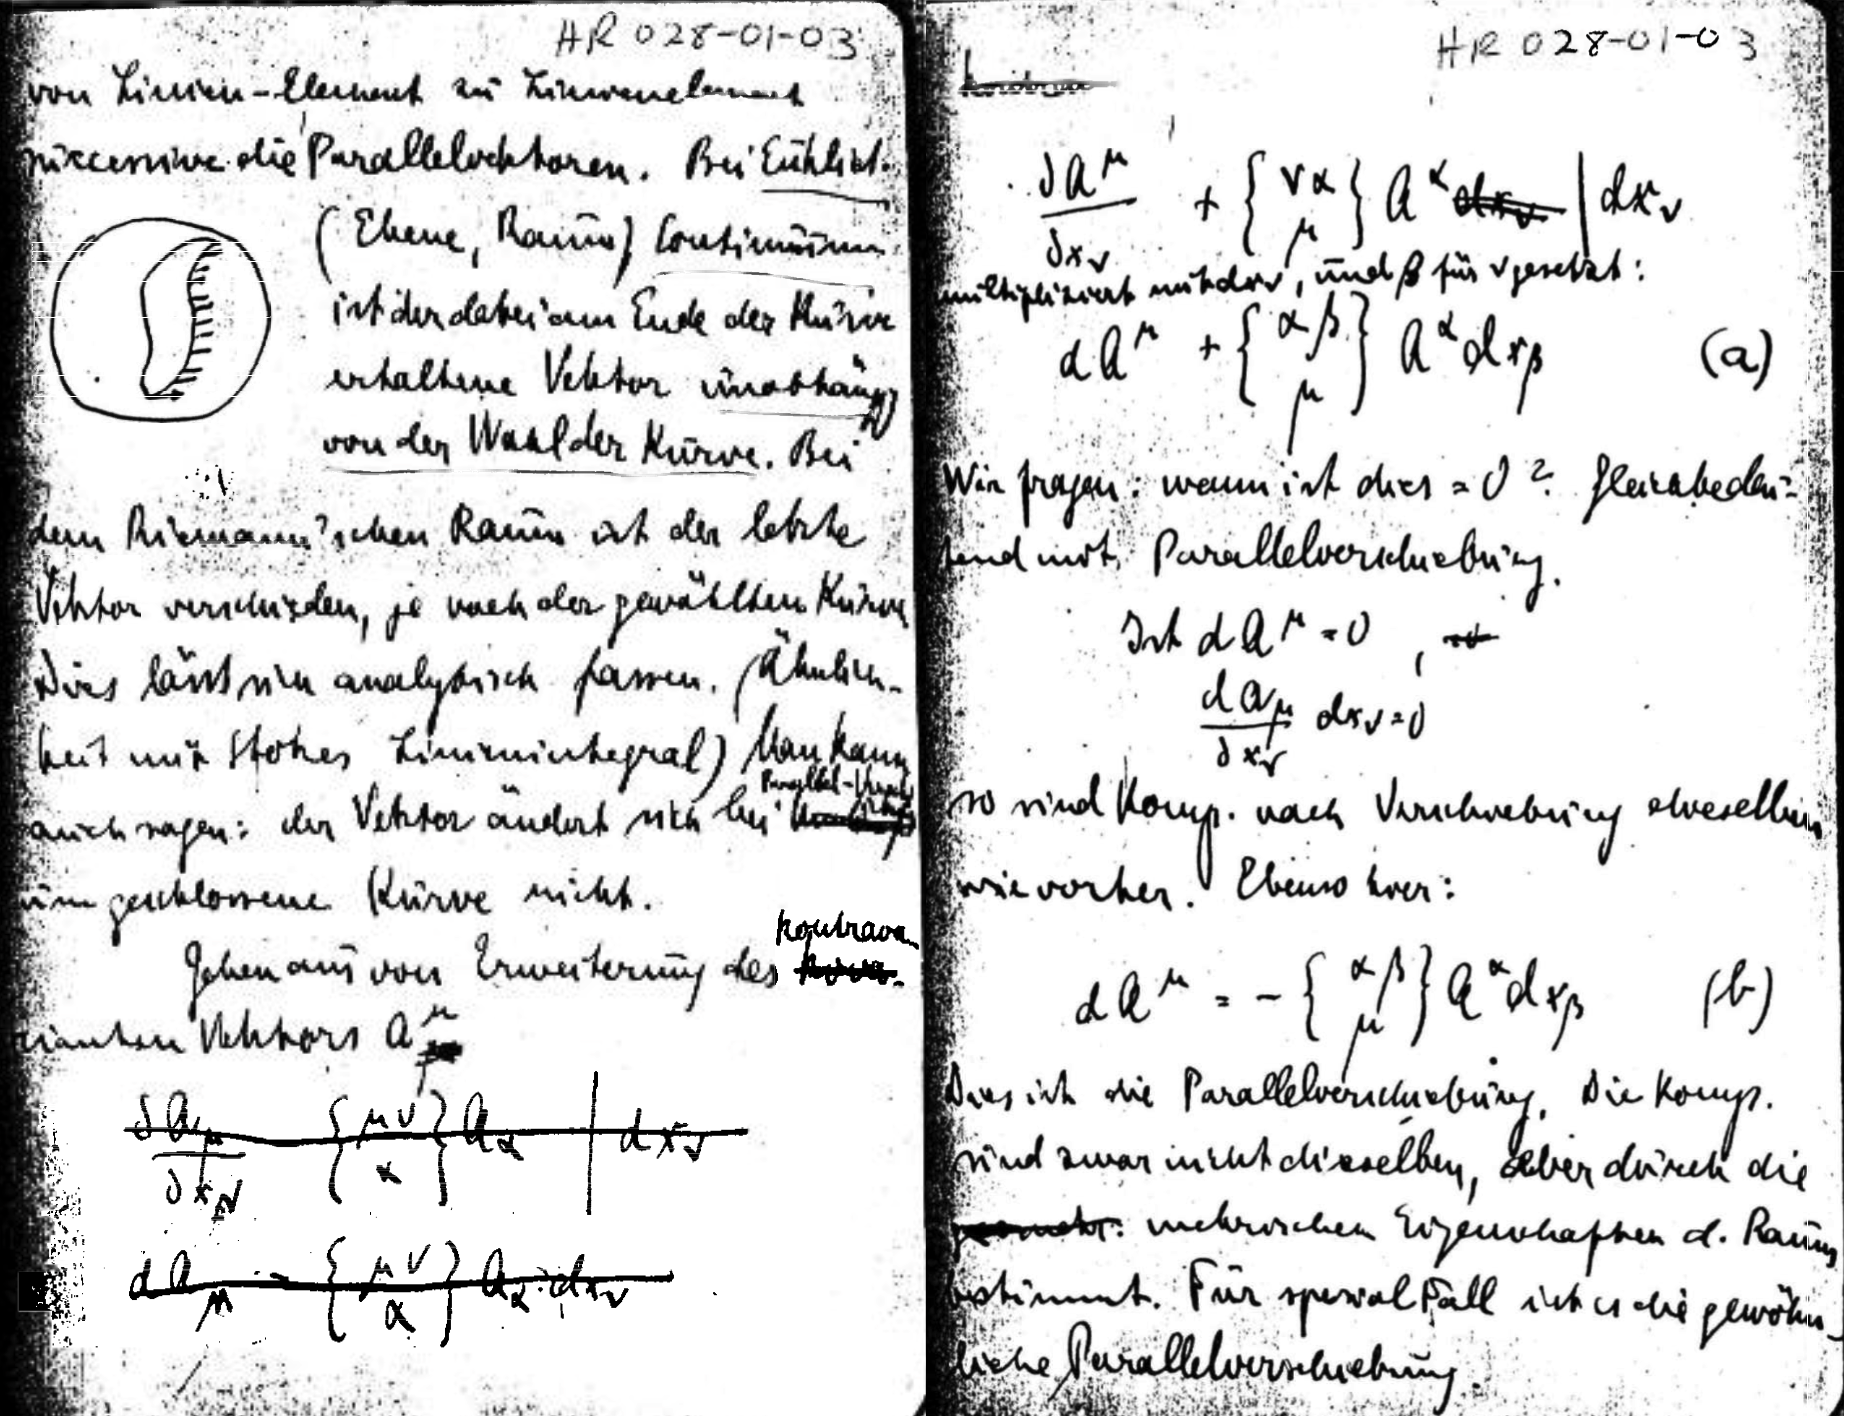
\includegraphics[scale=0.12, trim = 0mm 0mm 0mm 0mm, clip]{parallelverschiebungDOUB.png}
\caption{Reichenbach's student notes. Einstein introduces the notion of parallel transport of vectors}
\label{fig:parallel}
\end{center}
\end{figure}

This technical innovation in differential geometry played a fundamental role, not only in successive presentations of \gr \citep[see][]{Einstein1921}, but even more prominently in the development of the \uftp. If one starts with a symmetric \gmn, the road is, so to speak, marked. The Christoffel symbols are the only possible destination. However, if one defines the displacement \Gtmn independently of the metric \gmn, the Riemannian connection $\Gtmn = - \christoffel{\mu}{\nu}{\tau}$ appears only as a special case that has been achieved by introducing a series of conditions, that turned out not be necessary. By dropping some of these conditions, the possibility opens up to introduce additional mathematical degrees of freedom to accommodate the electromagnetic field alongside the gravitational field in a unified \scare{geometrical} description.

As it is well-known, \citet{Weyl1918a,Weyl1919a} was bothered by a conceptual asymmetry characterizing Riemannian geometry. The comparison of direction of vectors is path-dependent, whereas the comparison of their lengths remains distant-geometrical. To compensate for this  \scare{mathematical injustice} \citep{Afriat2009}, Weyl introduced a more general affine connection depending not only on the metric/gravitational tensor \gmn but also on the four-vector \phin. For formal reason, the latter could be identified with electromagnetic four-potential. \cop{Weyl could then conclude that, just like general relativity represented a geometrization of gravitational phenomena, his theory represented a unified geometrization of both gravitational and electromagnetic phenomena, which were, at that time, the only kind known}. Weyl did not hesitate to declare that \qt{Descartes' dream of a purely geometrical physics}{Der Traum des Descartes von einer rein geometrischen Physik} had be finally fulfilled \citep[263]{Weyl1919}.

Einstein had repeatedly criticized Weyl's attempt \citep{Einstein1918b}\todo{more examples}. However, by the spring of 1919, after a correspondence with Theodore Kaluza\todo{Kaluza} he had started to show increasing interest in the unification program \citep{Wuensch2005}. The question fell into the background after the success of the eclipse expedition was announced in November 1919 \citep{Dyson1920}. By the end of the year, Einstein was turned into an international celebrity, leaving him little time to work (\lettercpae{Einstein}{Fokker}{1}{12}{1919}[9][187], \lettercpae{Einstein}{Hopf}{2}{2}{1920}[9][295]). Inevitably, the German philosophical community started to show increasing interest in the theory \citep[see][for an overview]{Hentschel1990a}. The question whether the new theory was compatible with Kant's philosophy became particularly pressing. As a trained physicist with a doctorate in philosophy \cite{Reichenbach1916}, Reichenbach was in a privileged position to deal with this issue. By following Einstein's lectures, he had acquired a technical knowledge of the new theory that probably had no equal among the philosophers of his time. In February or March 1920, Reichenbach, who has just moved to Stuttgart, decided to write his habilitation on this topic \hide{Im Februar (oder März) 1920 beschloß ich, meine Habilitationsschrift zu schreiben}. \hide{Ich hatte in den Monaten vorher Relth. gearbeitet, auch nach Weyl; den Grund hatte ich schon 1917-1918}. In the preceding months, he had further worked on the theory \qt{also according to Weyl}{auch nach Weyl} \citep[044-06-23]{HR}---that is, probably studying Weyl's textbook \citetitle{Weyl1918} \citep{Weyl1918}. The Kapp-Pusch coup on \datemy{13}{3}{1920} gave Reichenbach a few days of leave from Huth radio industry, where he was employed \citep[044-06-23]{HR}. Thus, he could work without interruptions, and in ten days he completed an early draft. The manuscript was then typed and shown among others to Einstein. Thanks to the mediation of Arnold Berliner, the influential editor of the \jt{Naturwisseschaften}, Reichenbach obtained a publication agreement with Springer \citep[044-06-23]{HR}.



%11 Für weitere Ausführungen zur Entstehung von Relativitätstheorie und Erkenntnis apriori sei hier auf Kamlah 1979, Erläuterungen zu GW 3, 475-480; Maria Reichenbach, Vorwort zu Reichenbach 1965ü, The Theory of Relativity and A Priori Knowledge, xi-xliv oder Hentschel 1990, Interpretationen und Fehlinterpretationen….., 507-526 verwiesen.

Reichenbach's habilitation has recently attracted renewed attention \citep{Friedman2001}. Reichenbach borrowed from \citet{Schlick1918} that idea that physical knowledge is, ultimately (\emph{Zuordnung}), the process of relating an axiomatically defined mathematical structure to concrete empirical reality \citep{Padovani2009}. However, Reichenbach attempted  to give this insight a \scare{Kantian} twist. According to Reichenbach, in a physical theory, beside the \scare{axioms of connections} (\german{Verknüpfungsaxiome}) encoding the mathematical structure of a theory, one needs a special class of physical principles the \scare{axioms of coordination} (\german{Zuordnungsaxiome}) to ensure a univocal coordination of that structure to reality. For the young Reichenbach, the latter axioms are \apr in the sense that they are \scare{constitutive} of the object of a physical theory. However, they are not apodeictic, or valid for all time. As it is well known, Reichenbach would soon abandon the project of a constitutive but relativized \apr. However, he would firmly maintain \cop{the separation between the mathematical framework of a theory (the \scare{defined side}) and the way it related to empirical reality (the \scare{undefined side})} \rhp{40}{42} as an essential feature of his philosophy.


%Und drittens wurde von mathematischer Seite geltend gemacht, daß es sich in der Geometrie nur um konventionelle Festsetzungen, um ein leeres Schema handelte, das selbst keine Aussagen über die Wirklichkeit enthielte, sondern nur als ihre Form ge-wählt sei, und das mit gleichem Recht durch ein nicht· euklidisches Schema ersetzt werden könnte 1).

% theory as a example of a neglect to lessons to that mathematic alone could be the key to physical reality



%\cop{it has been \gr revealed the physical character of geometry as a science of real space, imposed the division of labor between pure and applied geometry}.  

%There are no references to \WT, however is roughly Reichenbach discuss with Einstein would whom he was clearly in friendly term. It is probably that Einstein might his skepticism\footnote{???}.

%few days in the spring of 1920.40 The manuscript, entirely available at the Pittsburgh Archives, was ready for publication, with minor modifications, during the summer of 1920. This material makes it clear that the distinction between axioms in these terms was inserted only later in revisions. Interestingly, in the drafts of this work there are traces of another specification in a marginal note, added later but eventually omitted from the published version. With respect to the passage of p. 54 that I have quoted above, Sect. 3.2, in this note he writes:


%The distinction between connecting and coordinating axioms has been understandbly regarded as a very striking version of the relativized a priori.38 In The Theory of



\subsection{Reichenbach's Habilitation and his critique of Weyl Theory}

According to Reichenbach, \rt made this division of labor in the realm of geometry inevitable. The possibility of non-Euclidean geometries had already indicated that the  Euclidean character of physical space could no longer been taken for granted \rhp{3}{3}. Mathematicians were inclined to considered geometry as an empty schema that did not contain any statements about the physical world, if not in the form of arbitrary conventions \rhp{3}{3}. In comparison to these positions, Reichenbach wrote, \q{the theory of relativity embodies a completely new idea} \rhp{3}{4}. \Rt claims that the theorems of Euclidean geometry do not apply to the physical space, that Euclidean geometry is simply \emph{false} \rhp{3}{4}. In this way, \rt has made necessary to \cop{distinguish between pure geometry as an uninterpreted formal system and applied geometry as an empirical theory of physical space} \rhp{73\todo{check}}{76}. The propositions of pure geometry are neither true nor false. The question of the truth of physical geometry pertain to physics alone. In order to clarify this point, rather in passing, Reichenbach, indicated \WT as a glaring example of how easy it was to slip into old habits. Weyl once again believed to have found a certain geometry that, for its intrinsic mathematical appeal, must have been true for physical reality: \qt{In this way the old mistake is repeated}{so begeht man nur den alten Fehler von neuem} \rhp{73}{76}.


%Wir gehen; jetzt zur allgemeinen Relativitätstheorie über. Sie behauptet, daß ein euklidischer Raum für die physikalische Wirklichkeit nicht angenommen werden darf. Wir fragen: welches.sind die Prinzipien und Erfahrungen, auf die sich die Theorie zur Begründung beruft? Warum nennt sie die Annahme eines euklidischen Raumes falsch?


%Euclid

%In this way does not challenge the validity of the Euclidean geometry but raised the question of its applicability to the physical space. It became inevitable to 

Reichenbach's brief outline of \WT is sufficient to grasp the gist of his argument. As Reichenbach's put it, \qt{Weyl's generalization of the theory of relativity  \textelp{} abandons altogether the concept of a definite length for an infinitesimal measuring rod}{Weylschen Verallgemeinerung der Relativitätstheorie 22) entgegengehalten werden, bei der der Begriff einer feststehenden .Länge für einen unendlich kleinen Maßstab überhaupt aufgegeben wird} \rhp{73}{76}. \cop{In Euclidean geometry a vector can be shifted parallel to itself along a closed curve so that upon its return to the point of departure it has the same direction and the same length. In the Einstein-Riemannian geometry it has merely the same length, no longer the original direction, after its return. In \WT it does not even retain the same length}. As we have seen, in this way, in addition to the \scare{metric tensor} \gmn, a \scare{metric vector} $\phin$ is introduced that, for formal reasons, could be identified with electromagnetic potential. Reichenbach conceded that \WT represented a possible generalization of Einstein's conception of \spti which, \qt{although not yet confirmed physically, is by no means impossible}{wenn auch physikalisch noch nicht bewiesen, doch auch keineswegs unmöglich ist} \rhp{76}{79}. 

Reichenbach seemed to have been aware of Einstein's main objection to Weyl's proposal \citep[see]{Einstein1918b}. In general relativity, the length $ds$ of the time-like vector $dx_\nu$ is measured by a physical clock, e.g., by the crests of waves of radiation were emitted by an atom. If we maintain this interpretation, then Weyl's theories implies that \q{the frequency of a clock is dependent upon its prehistory}{Nach der Weylschen Theorie ist die Frequenz einer Uhr von mrer Vorgeschichte abhängig.} \rhp{77}{80}. Two atomic clocks, at one place, will in general not tick at the same rate when they are separated brought back together. This result appears to be contradicted by a vast amount of spectroscopic data shown that all atoms of the same type have the same systems of stripes in their characteristic spectra independently of their past history. Reichenbach conceded to Weyl that these effects might \q{compensate each other on the average}daß sich diese Einflüsse im Durchschnitt ausgleichen, \rhp{77}{80}. Thus, the fact that \qt{the frequency of a spectral line under otherwise equal conditions is the same on all celestial bodies}{Frequenz einer Spektrallinie bei sonst gleichen Umständen auf allen Himmelskörpern gleich ist, als Näherungen
erklären} could he interpreted as an approximation, rather than being a consequence of the Riemannian nature of space-time \rhp{77}{81}. This remark anticipates to a certain extent Weyl's line of defense. However, Reichenbach considered unacceptable was Weyl's justification for the choice of a more general geometry as the actual geometry of \spti.

According to Reichenbach, Weyl seems to imply that his non-Riemannian geometry must be true \emph{physically} because it is \emph{mathematically} superior to Riemannian geometry, being the true realization of the principle of locality. As we have seen, in Weyl geometry a vector moving close loop which would same length but different direction in Riemannian geometry, different length and different direction in Weyl's geometry. Thus, Weyl geometry eliminated the last distant-geometrical treatment of Riemannian geometry. Weyl geometry seems to be the most \scare{general geometry}, a purely infinitesimal geometry. Thus, there would be no reason to assume from the outset that a more special geometry applies to reality. However, Reichenbach had already surmised that this generalization could be continued. In Weyl geometry lengths can be compared at the same point in different directions, but not at distant points. \qt{The next step in the generalization would be to assume that the vector changes its length upon turning around itself}{Die nächste Stufe der Verallgemeinerung wäre die, daß auch bei der Drehung um sich selbst der V ektor bereits seine Länge geändert. hat} \rhp{76}{85}. Probably, more complicated generalizations could be thought of. \qt{Nothing may prevent our grandchildren from being confronted some day by a physics that has made the transition to a line element of the fourth degree}{ichts könnte unsere Enkel davor schützen, daß sie eines Tags vor einer Physik stehen, die zu einem Linienelement vom vierten Grade übergegangen is} \rhp{76}{79}\footnote{$d s^{4}=g_{\mu \nu \sigma \tau} d x_{\mu} d x_{\nu} d x_{\sigma} d x_{\tau}$ instead of $d s^{2}=\gmn d x_{\mu} d x_{\nu}$ as in Riemannian geometry}. Thus, there is no \q{\scare{most general} geometry} that in and by itself must be physically true \rhp{76}{80}. No matter one pushes further the level of mathematical abstraction, the \q{difference between physics and mathematics}  \rhp{76}{80} cannot be erased; geometry alone can never be sufficient to establish the reality of physical space \rhp{76}{80}. 

Thus, Reichenbach accused Weyl of having neglected the main philosophical lesson of \gr, the unbridgeable difference between physics and mathematics. A mathematical axiom system is indifferent with regard to the applicability and \q{never leads to principles of an \emph{empirical theory}} \rhp{73}{76}. \qt{Only a physical theory could answer the question of the validity}{Erst eine physikalische Theorie konnte die Geltungsfrage des euklidischen Raumes beant-worten} \rhp{73}{76} of a particular geometry for physical space:

\qt{[Thus] it is incorrect to conclude, like Weyl\footnote{\cite[227]{Weyl1918}. In the 1919 edition of the \citetitle{Weyl1918} Weyl included a presentation of his theory. Thus, conclusion was characterized by even more inspired rhetoric: \q{physics and geometry coincides with each other} \citep[263]{Weyl1919}. The tendency of physicalizing geometry that have prevailed leading protagonists of the 19th century from Gauss to Helmholtz seemed to superseded have of geometrizing physics that run from Riemann to Einstein: \q{geometry has not been physics but physics has become geometry} \citep[263]{Weyl1919}} and Haas\footnote{\cite{Haas1920}}, that mathematics and physics are but one discipline. The question concerning the \emph{validity} of the axioms for the physical world must be distinguished from that concerning \emph{possible} axiomatic systems. It is the merit of the theory of relativity that it renowned the question of the truth of geometry from mathematics and relegated it to physics. If now, from a general geometry, theorems are derived and asserted to be a necessary foundation of physics, the old mistake is repeated. This objection must be made to Weyl's generalization of the theory of relativity \textelp{} Such a generalization is possible, but whether it is compatible with reality \myemph{does not depend on its significance for a general local geometry}. Therefore, Weyl's generalization must be investigated from the viewpoint of a physical theory, and only experience can be used for a critical analysis. Physics is not a \scare{geometrical necessity}; whoever asserts this returns to the pre-Kantian point of view where it was a necessity given by reason \rhp{73}{76}}{Ganz falsch ist es aber, wenn man daraus, wie z. B. Weyl und auch Haa.s tt), wieder den Schluß ziehen will, daß Mathematik und Physik zu einer einzigen Disziplin zusammenwachsen. Die Frage der Geltung von Axiomen für die Wirklichkeit und die Frage nach den möglichen Axiomen sind absolut zu trennen. Das ist ja gerade das
•
Verdienst der Relativitätstheorie, daß sie die Frage der
Geltung der Geometrie aus der Mathematik fortge- nommen und der Physik überwiesen hat. Wenn man jetzt aus einer allgemeinen Geometrie wieder Sätze aufstellt und behauptet, daß sie Grundlage der PJ.iysik sein müßten, so begeht man nur den alten Fehler von neuem. Diest:r Einwand muß der Weylschen Verallgemeinerung der Relativitätstheorie 22) entgegengehalten werden, bei der der Begriff einer feststehenden .Länge für einen unendlich kleinen Maßstab überhaupt aufgegeben wird. Allerdings ist eine solche Verallgemeinerung möglich, aber ob sie mit der Wirklichkeit verträglich ist, hängt nicht von ihrer Bedeutung für eine allgemeine Nahegeometrie ab. Darum muß die Weylsche Verallgemeinerung vom Standpunkt einer physikalischen Theorie betrachtet werden, und ihre Kritik erfährt sie allein durch die Erfahrung. Die Physik ist eben ~eine „geometrische Notwendigkeit"; wer das behauptet, kehrt auf·den vorkantischen Standpunkt zu ück, wo sie eine vernunftgegebene Notwendigkeit war}. 
%
To a certain extent, this objection contains the backbone of Reichenbach's criticism of the \uftp in the following decade. Weyl seems to have misunderstood the fundamental lesson of Einstein's theory. The question of the \q{\emph{validity} of axioms for the physical world} \rhp{73}{76} must be distinguished from that concerning possible axiomatic systems happened to be in reality. It is true that it is \q{a characteristic of modern physics to represent all processes in terms of mathematical equations}, and, one might add, progressively more abstract mathematics. Still, \q{the close connection between the two sciences must not blur their essential difference} {impliziten Definitionen}. The truth of mathematical propositions depends upon internal relations among their terms; the truth of physical propositions, on the other hand, depends on relations to something external, on a connection with experience. \qt{This distinction is due to the difference in the objects of knowledge of the two sciences}{Es ist das Kennzeichen der modernen Physik, daß sie alle Vorgänge durch mathematische Gl~ichiingen darstellt; aber diese Berührung zweier Wissenschaften darf über. deren grunds~tzlichen Unterschied nicht hinweg-täuschen} \rhp{33}{34}. The mathematical object of knowledge is uniquely determined by the axioms and definitions of mathematics. The definitions indicate how a term is related to that \citet{Schlick1918} had called \qt{implicit definitions}{impliziten Definitionen} \rhp{33}{36}. 

As it is well-known, Reichenbach will abandon the Kantian framework in which this distinction was initially presented. However, he never abandoned the idea that the separation between mathematics and physics was of paramount epistemological importance: mathematical necessity must be sharply distinguished from physical reality. This separation was the irreversible conceptual shift that \rt had forced upon philosophy. On \datef{24}{6}{1920}, Einstein praised Reichenbach's \german{Habilitationschrift} in a letter to Schlick \lettercpaep{Einstein}{Schlick}{19}{4}{1920}[9][378]. A few days later, Reichenbach asked Einstein to dedicate the book to him, insisting on the philosophical significance of \rt:  \qt{very few among tenured philosophers have the faintest idea that your theory performed philosophical act and that your physical conceptions contain more philosophy than all the multivolume works by the epigones of the great Kant}{Philosophen eine Ahnung davon haben, dass mit Ihrer Theorie eine philosophische Tat getan ist, und dass in Ihren physikalischen Begriffsbildungen mehr Philosophie enthalten ist, als in allen vielbändigen Werken der Epigonen des grossen Kant} \lettercpaep{Reichenbach}{Einstein}{13}{6}{1920}[10][57]. Einstein conceded, that the theory might have had philosophical relevance: \qt{The value of the th.\ of rel.\ for philosophy seems to me to be that it exposed the dubiousness of certain concepts that even in philosophy were recognized as small change \origins{Scheidemünzen}}{Der Wert der Rel.Th. für die Philosophie scheint mir der zu sein, dass sie die Zweifelhaftigkeit gewisser Begriffe dargethan hat, die auch in der Philosophie als Scheidemünzen anerkannt waren}  \lettercpaep{Einstein}{Reichenbach}{30}{6}{1920}[10][66]. Alleged \apr principles are like those parvenu that are ashamed of their humble origin and try to deny it: \qt{[c]oncepts are simply empty when they stop being firmly linked to experience}{Begriffe sind eben leer, wenn sie aufhören, mit Erlebnissen fest verkettet zu sein} \lettercpaep{Einstein}{Reichenbach}{30}{6}{1920}[10][66]\footnote{Einstein used a similar wording by commenting on the manuscript of Cassirer's \scare{Kantian} booklet on relativity. \q{Conceptual systems appear empty to me, if the manner in which they are to be referred to experience is not established} \lettercpaep{\Einstein}{\Cassirer}{6}{6}{1920}[10][44]. In particular, \q{[w]ith the interpretation of the $ds$ as a result of measurement, which is obtainable by means of measuring rods and clocks the general theory of relativity as a physical theory stands or falls} \lettercpaep{\Einstein}{\Cassirer}{6}{6}{1920}[10][44]. The gravitational redshift, can be taken as an empirical confirmation of general relativity only because different atoms of the same substance can be regarded as identically constructed clocks reproducing the identical unit of time. For this reason, it is possible to \scare{normalize} the absolute value of $ds$ by counting the wave crests on atom. According, \WT deprived the $ds$ of any physical meaning. However, real \rac behave differently than predicted by \WT forcing Weyl to assume an inconsistent position. According to Einstein, line \gr, Weyl's  \q{theory is based on a measuring rods geometry}, that is, it presupposes the comparability of lengths. However, it pertains only \q{thought measuring rods \origins{nur gedachte Massstäbe}} that behave differently from the real ones. \q{This is repugnant} \lettercpaep{\Einstein}{\Besso}{26}{8}{1920}[10][85\me]}. This remark, which Reichenbach would later quote in a published writing \citep[354]{Reichenbach1922a}, seals a sort of philosophical alliance between Reichenbach and Einstein. Against the Weyl's speculative style of doing physics which reduced physical reality to geometrical necessity, \rt had has introduced a clear-cut separation between geometrical necessity and physical reality. As we shall see, this philosophical covenant will be broken less than a decade later.

%Sie gleichen Emporkömmlingen, die sich ihrer Abstammung schämen und sie verleugnen wollen

\subsection{The Reichenbach-Weyl Correspondence}
%EC an Hans Reichenbach, Hamburg 02. 07. 1920, 2 S., Pittsburgh. 285 EC an Hans Reichenbach, Hamburg 07. 07. 1920, 2 S., Pittsburgh.

Reichenbach's book was published a few months later, just on that occasion, the 86th Assembly of the \german{Versammlung der Gesellschaft Deutscher Naturforscher und Ärzte} in Bad Nauheim in September 1920. This meeting of fundamental importance for in the history of \rt, not least for the famous debate between Einstein and Philipp Lenard \citep{Dongen2007}. Reichenbach met Weyl there for the first time, where the latter gave a talk on his unified theory \citep{Weyl1920}. Reichenbach might have assisted at the debate that followed, in which Einstein rehearsed his objections against Weyl\footnote{Commenting on Weyl's talk, he pointed out once again that the \q{arrangement of \textins{his} conceptual system,} \q{it has become decisive \origins{massgebend} to bring elementary experiences into the language of signs \origins{Zeichensprache}} \citep[650]{Einstein1920c}. For Einstein, \q{temporal-spatial intervals are physically defined with the help of measuring rods and clocks}, under the assumption that \q{their equality is empirically independent of their prehistory} \citep[650]{Einstein1920c}. Einstein insisted that precisely upon this assumption rests \q{the possibility of coordinating \origins{zuzuordnen} a number $ds$ to two neighboring world points}; if this were impossible, general relativity would be robbed of \q{its most solid empirical support and possibilities of confirmation} \citep[650]{Einstein1920c}.
}, and the same time defended the possibility of a field theory of matter against Pauli's objections\footnote{In is interesting to notice, that Einstein already showed a more flexible attitude replying to Pauli's remarks during the same discussion. \Pauli reiterated his objection based on his \scare{observability} criterion. Just as the field strength in the interior of the electron is meaningless because there is no smaller test particle than the electron, \q{one could claim something similar concerning spatial measurements, \myemph{since there are no infinitely small measuring-rods}} \citep[650]{Einstein1920c}. Einstein replied to \Pauli that \q{with the increasing refinement of the system of scientific concepts, the manner and procedure of associating the concepts with experiences becomes increasingly more complicated} \citep[650]{Einstein1920c}. In particular, he recognized that in cases such as that of the continuum theories, \q{one finds that a definite experience cannot be associated any longer with a concept} \citep[650]{Einstein1920c}. According to Einstein, there is an alternative: one can abandon \scare{continuum theories} for the sake of \Pauli's observability criterion, or replace such a \q{system of associating concepts \textins{with experiences} with a more complicated one} \citep[650]{Einstein1920c}.  Einstein's in his contributions to the the discussion which followed Max von \citets{Laue1920}'s Bad Nauheim paper. Einstein, however, in the very same sentence, did not hesitate to admit that \q{[it] is a logical shortcoming of the theory of relativity in its present form to be forced to introduce measuring rods and clocks \myemph{separately instead of being able to construct them as solutions to differential equations}} \citep[Einstein's reply to][662\me]{Laue1920}}.  Schlick did not attend Bad Nauheim but received Reichenbach's new published book in those days. Writing to Einstein, he praised the book, but complained about his critique of conventionalism \lettercpaep{Schlick}{Einstein}{23}{9}{1920}. 

The five letters that Reichenbach exchanged with Schlick between October and November 1920\footnote{\letterhr{Schlick}{Reichenbach}{25}{9}{1920}[015-63-23]
\letterhr{Schlick}{Reichenbach}{26}{11}{1920}[015-63-22]
\letterhr{Schlick}{Reichenbach}{11}{12}{1920}[015-63-19]
\lettersa{Reichenbach}{Schlick}{29}{11}{1920}
\lettersa{Reichenbach}{Schlick}{10}{9}{1920}} turned out to be of fundamental importance in his intellectual biography. Reichenbach was confronted with Schlick's objection that his \scare{axioms of coordination} were nothing but \scare{conventions}. He initially opposed some resistance. If the coordinating principles are fully arbitrary, he feared, geometry would be empirically meaningless. In Poincaré' conventionalism, Reichenbach missed  claim that \qt{the arbitrariness of the principles is constrained, if the principles are combined}{daß die Willkürlichkeit der Prinzipien eingeschränkt ist, sowie man Prinzipien KOMBINIERT} \letterhr{Reichenbach}{Schlick}{26}{11}{1920}[015-63-22]. Einstein's famous lecture on \scare{geometry and experience} of the end \datemy{27}{1}{1921} \citetitle{Einstein1921}\footnote{Most readers seems to have neglected that the problem that the lecture was discussing was related to the Bad Nauheim's discussion with Weyl and Pauli. On \datef{14}{1}{1921} Einstein, while in Vienna, released the following declaration: \qt{A theoretical system can only claim completeness if the relationships of the concepts to the facts that can be experienced are clearly established. It is not enough, for example, to base the theory of relativity on a mathematical fundamental invariant [$ds$]. It must also be clear how this invariant is related to the observable facts as [that](2) [happened] for the fundamental concepts of Maxwell's theory by Heinrich Hertz. If one disregards this point of view, one can only arrive at unrealistic systems}{Wenn ich die gegenwärtige Lage der theoretischen Physik überschaue, so scheint mir ein Punkt von großer Wichtigkeit nicht hinlänglich beachtet zu werden. Ein theoretisches System kann erst dann Vollständigkeit beanspruchen, wenn die Beziehungen der Begriffe zu den erlebbaren Tatsachen eindeutig festgelegt sind. Es genügt zum Beispiel nicht, die Relativitätstheorie an eine mathematische auf eine mathematische Fundamentalinvariante zu gründen. Es muß auch klar sein, wie diese Invariante mit den beobachtbaren Tatsachen zusammenhängt wie [das](2] für die Fundamentalbegriffe der Maxwellschen Theorie durch Heinrich Hertz [geschehen ist.] Läßt man diesen Gesichtspunkt außer acht, SO kann man nur zu wirklichkeitsfremden Systemen gelangen} \CPAEp{7\textins{13}}{50a} A few days later \datef{27}{1}{1921} Einstein held \citetitle{Einstein1921} in Berlin. the lecture ultimately meant to address precisely this issue, although in a popular form. (a) the invariant $ds$ is measured by ideal \rac, like the electric field strengths are measured by charged test particles (b) ideal \rac do not exist in nature (as pointed out by Poincaré). Conclusion: \emph{sub specie aeterni} geometry cannot be tested separately from the rest of physics (the famous $G+P$ formula). The choice of a particular geometry is ultimately justified by its success of delivering a good physical theory. It is assumed that solutions to the appropriate dynamical equations exist that can serve as \rac. In \WT, however, real \rac would behave differently from the ideal \rac in Weyl geometry. This inconsistency was the point that Einstein found unbearable. Thus, in March 1921 Einstein preferred to suggest a theory in which there were no transportable ideal rods at all and only $ds=0$ has physical meaning \citep{Einstein1921c}} seemed to have tipped the scale in Schlick's favor \citep[5]{Reichenbach1921a}. At the beginning of the lecture, Einstein mentions approvingly Schlick's separation between pure and applied geometry.  He provisionally defended a form of geometrical empiricism in which geometry has physical meaning separately from physics if understood as the science of the behavior of rigid rods. However, since perfectly rigid rods do not exist in nature, geometry seems to lose gain its connection with reality. As a way out, Einstein pleaded for a holistic reading of Poincaré's conventionalism. Geometry isolated might be arbitrary, but the combination $(G)$eometry+$(P)$hysics has an empirical meaning \citep[5]{Reichenbach1921a}\footnote{\citet{Reichenbach1922a} seems to have ultimately turned the Einstein's $G+P$ formula into his $G + F$ formula, where $F$ is a \scare{metric force} affecting all bodies in the same way. By setting $F=0$ geometry becomes empirically testable. Reichenbach could embrace conventionalism, without having to accept that the proposition of geometry are empirical meaningless}.



%Indeed, there not only Einstein seems to defend conventionalism, but also offered the possibilities of avoiding the 

% Dingler



% Schlick position of the separation between mathematics and physics, which will be ulitately sanctioned by Einstein's himself in this famous lecture of Jarnaury 1021.

%That Einstein seemed to have then that the coordination could be directly with \rac. It is true that Einstein seemed to have a more geneours will be valid in principles. However, logical empiricists clearly interpreted as improved version of conventionalism, not simplicity by of geometry and physics. In this way, was bale to embrace conventionalism, that indeed to assure the univocality of coordination.

%ne objektive Eigenschaft der Wirklichkeit beschreibt

%Dann enthält auch der Vergleich zweier kleiner Maßstäbe an verschiedenen Punkten des Raumes keine objektive Relation mehr

Reichenbach must have sent a copy of his \citetitle{Reichenbach1920a} \citep{Reichenbach1920a} also to Weyl despite the rather severe critiques he had expressed in the book. Weyl replied with some delay in \datemy{2}{2}{1921}. He did  not appear to be upset by Reichenbach's objections, and replied rather amicably to some issues \q{which concern less the philosophical than the physical} \letterhrp{Weyl}{Reichenbach}{2}{2}{1921}[015-68-04]. In particular, Weyl denied having ever claimed that physics has been absorbed into mathematics:

\qt{It is certainly not true, as you say on p.\ 73, that, for me, mathematics (!!, e.g. theory of the $\zeta$-function?) and physics are growing together into a single discipline. I have claimed only that the \emph{concepts} in \emph{geometry} and field physics have come to coincide \textelp{} As for my extended theory of relativity, so I cannot admit that the epistemological situation is in any way different from that of Einstein. \textelp{} \emph{Experience} is in no way anticipated by the assumption of that general metric; that the laws of nature, to which the propagation of action in the ether is bound, can be of such a nature that they do not allow any curvature. \textelp{} What I stand for is simply this: The integrability of length transfer (if it exists, but I don't think so, because I don't see the slightest dubious reason for it) does not lie in the nature of the metric medium, but can only be based on a special law of action\footnote{That is on the field equations of the theory which in turned can be derived from an \scare{action principle}}. If the historical development had been different, it seems to me that no one would have thought of considering the Riemannian case from the outset. As far as the notorious \scare{dependence on previous history} is concerned, I probably expressed my opinion clearly enough in Nauheim \letterhrp{Weyl}{Reichenbach}{2}{2}{1921}[015-68-04]}{ Was nıeine erweiterte Relativitätstlıeorie betrifft. so kann ich nicht zugeben, daß da erkenntnislogisch die Sache irgendwie anders liegt wie bei Einstein. \textelp{}  Der Erfahrung wird durch die Annahme jener allgemeiner Metrik in keiner Weise vorgegriffen; dass die Naturgesetze, an welche die Wirkungsausbreituug in Äther gebunden ist, können ja von solcher Art sein, daß sie keine Streıfkenkrümmung zulassen. \textelp{} Wofür ich allein eintrete, ist dies: Die Integrabilität der Strekken\"ubertraguug (wenn sie besteht, ich glaubs uielıt. denn ich sehe nicht den geriugsteu zwiugeudeu Grund dafür) liegt uielıt im Wesen des metrischen Mediumsm, sondern kann nur auf einem besonderen Wirkungsgesetz berulıen. Ware die historische Entwieklung anders verlaufien, so seheint nıir wåire uienıand darauf verfallen. von vorn- herein gerade nur den Rieuıauuselıeu Fall iu Erwåígımg zu zielıeu. - *Nas die berüchtigte “Abhšingigkeit von der Vorgeschichte" betrifft, so habe ieh darüber wohl nıeine Ansicht deutlieh gemıg in Naulıeinı ausgesprochen. An der 4. Aufl. wird Sie wahrscheinlich vor al- lenı nıeine veränderte Stellımgnalnue zum Problem der Materie i}
%
In Bad Nauheim, Weyl outlined a now well-known speculative explanation for the discrepancy between the behavior of \scare{ideal} and \scare{real} rods. Roughly, Weyl suggested that the atoms we use as clocks might not \emph{preserve} their size if transported, but \emph{adjust} it every time to some constant field quantity, which he could identify with the constant radius of the spherical curvature of every three-dimensional slice of the world \citep{Weyl1920a}. The geometry read off from the behavior of material bodies would appear different from the actual geometry of \spti, because of the \scare{distortion} due to the mechanism of the adjustment. In 1921, the \scare{pivotal year} for unified field theories \citep[ch.\ 4]{Vizgin1994}, \Weyl (followed to some extent by \cite{Eddington1921,Eddington1921a}) reacted by expanding his strategy of \scare{doubling the geometry}, the real \scare{aether geometry} and the \scare{body geometry} distorted by the mechanism of adjustment\footnote{A different variation of this strategy of doubling the geometry was suggested by Eddington at about the same time. He considered non-Riemannian geometries as mere \scare{graphical representation} that might serve to organize different theories into a common mathematical framework. The \q{natural geometry} remains exactly Riemannian \citep{Eddington1921}}, in three papers intended for different audiences, February \citep{Weyl1921a}, May \citep{Weyl1921d} and July \citep{Weyl1921e}. In the July paper, Weyl also addresses Reichenbach's criticism publicly:

\qt{From different sides\footnote{The reference is to \citealp{Reichenbach1920a} and \citealp{Freundlich1920} who, however, refers to \cite{Haas1920}} it has been argued against my theory that it would attempt to demonstrate in a purely speculative way something \emph{a priori} about matters on which only experience can actually decide. This is a misunderstanding. Of course from the epistemological principle \origins{aus dem erkenntnistheoretischen Prinzip} of the relativity of magnitude does not follow that the \scare{tract} displacement \origins{Streckenübertragung} through \scare{congruent displacement} \origins{durch kongruente Verpflanzung} is not integrable; from that principle that no \emph{fact} can be derived. The principle only teaches that the integrability \emph{per se} must not be retained, but, if it is realized, it must be understood as the \myemph{outflow \origins{Ausfluß} of a law of nature} \citep[475; last emphasis mine]{Weyl1921b}}{3. Von verschiedenen Seiten?) ist gegen meine Theorie eingewendet worden, daß in ihr aus reiner Spekulation Dinge a priori demonstriert würden, über .welche nur die Erfahrung entscheiden kann. Das is ein Mißverständnis. Aus dem erkenntnistheoretischen Prinzip von der Relativität der Größe folgt natürlich nicht, daß die Streckenübertragung durch kongruente Verpflanzung nicht integrabel ist; es folgt aus ihm überkaupt keine-Tatsache. Es lehrt nur, daß Integrabilität an sich nicht zu bestehen braucht, sondern, wenn sie stattfindet, als Ausfluß eines Naturgesetzes verstanden werden muß}
%
As Weyl explains in this passage, he never claimed that his geometry entails in its mathematical structure alone the \apr justification of its physical truth. On the very contrary, he questioned the alleged \apr status of the assumption that the comparison of lengths is path-independent. For this reason, Weyl did not deny the well-established \cop{empirical fact that two atoms of the same chemical substance placed identically in the same conditions, is independent of their prehistory}. However, he insists that the physical behavior of atoms does not have anything to do with the abstract notion of parallel transport of vectors\footnote{\label{pauli}In September 1921, Pauli's encyclopedia article on relativity theory was published, as part of the fifth volume of the \bt{Enzyklopädie der Mathematischen Wissenschaften}, and later as a book with an introduction by Pauli's mentor, Arnold Sommerfeld \citep{Pauli1921}. In the chapter dedicated to \WT, Pauli suggested that Weyl provided two different versions of the theory. In the first version \WT sought to make predictions on the behavior of \rac, just like Einstein's theory. From this point of view, the theory is empirically inadequate because of the existence of atoms with sharp spectral lines. Later, Weyl renounced this interpretation. The ideal process of the congruent displacement vectors has nothing to do with the real behavior of \rac \citeptra[763]{Pauli1921}[196]{Pauli1958}. However, in this form the theory furnishes only \q{formal, and not physical, evidence for a connection between \textins{the} world metric and electricity} \citeptra[763]{Pauli1921}[196]{Pauli1958}. In this form, the theory loess its \q{convincing power \origins{Uberzeugunggkraft}} \citeptra[763]{Pauli1921}[196]{Pauli1958}}. Einstein simply assumed as empirical fact the ratio of the wave lengths of two spectral lines is a  physical constant that can be used to normalize the $ds$. Weyl, on the contrary, claims that the wave lengths of two spectral lines are always a multiple of a certain field quantity of dimension of a length that can be used to normalize the $ds$. Nevertheless, the constancy of emerged from a theory in which only the ration of $ds$ at a point is physically meaningful.

\subsection{The Weyl-Reichenbach Appeasement}

\hide{Im Sept. 1921 trug ich schon den ersten Bericht \"uber die Axiomatik auf dem Physikertag in .lena vor.3 Ich hatte damals gro§en Erfolg; aber niemand ist damals auf den Gedanken gekommen, mich in eine angemessene Stelle zu berufen. Ich blieb in Stuttgart sitzen. Niederschrift und Ausbau im Winter 1921 /22.}  \hide{Niederschrift und Ausbau im Winter 1921/22. Das alte MS wurde völlig umgestoßen. Genauere Behandlung der allg. Th. im Aug.-Spt. 1922. Vortrag darüber in Leipzig, Sept. 1922.}

Weyl's paper referencing Reichenbach appeared at the beginning of September \citep{Weyl1921e}. A few weeks later, Reichenbach and Weyl met again in Jena on occasion of the first  \german{Deutsche Physiker- und Mathematikertag}, the first national scientific meeting held independently from the meetings of the \textit{Gesellschaft Deutscher Naturforscher und Ärzte}. Weyl gave a talk in which he tried to provide a mathematical justification for the quadratic or Pythagorean nature of the metric \citep{Weyl1921f}\footnote{I assume that this talk would have again bee suspiction since the local is intrinsically mathematical reason. Indeed, in Reuchenbach view there was no reason}. Reichenbach presented a report of his work on the axiomatization of relativity \citep{Reichenbach1921d}. This report is the first written testimony of the development of Reichenbach's philosophy after the Schlick-correspondence. Reichenbach suggested that in a physical theory one should distinguish the \emph{axioms} as empirical proposition about light rays, \rac\etc and the \emph{definitions} that establish the conceptual framework of the theory \lettercpaep{Reichenbach}{Einstein}{5}{12}{1921}[12][266]. After the paper came out by the end of the year \citep{Reichenbach1921d}, Reichenbach must have sent a copy to Weyl in a lost letter of \datef{8}{1}{1922}. He might have included a personal retraction of his criticisms. However, the letter is no longer extant and reached Weyl only months later, \letterhrp{Weyl}{Reichenbach}{3}{3}{1922}[015-68-03] since he was in Barcelona, where he was giving his Catalonian Lectures \citep{Weyl1923}.

However, Reichenbach soon issued a public retraction. In those months, he was working on a long review article about philosophical interpretations of relativity, that he finished in Spring 1922. In March, Erwin Freundlich sent the proofs of the paper  to Einstein \lettercpaep{Freundlich}{Einstein}{24}{3}{1922}[13][109], who \cop{expressed his general agreement with Reichenbach's analysis of the philosophical implications of relativity and praised its clarity} \lettercpaep{Einstein}{Reichenbach}{27}{3}{1922}[13][119]. The paper reviews the most significant philosophical interpretation of relativity. However, it also included a last section on Weyl's \uft: \q{One cannot conclude an exposition of relativistic philosophy}, Reichenbach wrote \qt{without considering the important expansion that Weyl bestowed on the problem of space three years ago}{Man darf eine Darstellung der relativistischen Philosophie nicht abschließen, ohne der wichtigen Erweiterung zu gedenken, die vor 3 Jahren Weyl dem Raumproblem zuteil werden ließ} \citep[365]{Reichenbach1922a}.

%\footnoteh{Reality does not unambiguously prescribe one geometry and that, in choosing the definition of congruence, we have it in our power to determine the nature of the geometry that will subsequently emerge. A deviation from Euclidean geometry, then the preceding argument means that we must interpret this deviation as action of a force that deforms the measuring rods; but to admit the existence of such universal forces in physics would be to introduce uncertainty into all practical measurements. By excluding this kind of forces from the outset one fixed the definition of geometry. This was for Reichenbach essentially the proposition that only physics and geometry taken together as a whole is subject to the test of experience. As we shall see this was probably not Einstein's intention. Indeed, atomic clocks there is littler room for decision}

%A deviation from Euclidean geometry, then the preceding argument means that we must interpret this deviation as action of a force that deforms the measuring rods. In a thermostatic umiverse iron rods and copper rods form two distinct classes of rigid rods.  For a given temperature distribution over space, the metric depends on the kind of rod used. However, das ist ja auch der Sinn des Konventionalis- :mus.

Reichenbach appears to be now fully converted to conventionalism. The choice between Euclidean and non-Euclidean geometries is conventional, that is, it depends on which rods are rigid. \citep[366]{Reichenbach1922}. However, both Euclidean and non-Euclidean geometries tacitly presuppose the validity of an axiom based on an empirical fact: rods that are of equal length in one place can be obtained in one place, it will be possible at any other places, no matter how the prehistory of each rod might have been. If this were not the case, a different definition of the unit of length would have to be given for every space point. Reichenbach labels this tacit assumption the \qt{axiom of the Riemann class}{Axiom der Riemannklasse} \citep[366]{Reichenbach1922}. 

The merit of Weyl is to have shown that this axiom, although quite natural, is not necessary and can be questioned: From this point of view, what Weyl achieved is a purely mathematical discovery; it indicates a more general type of manifold that can be applied to reality when the Riemann class of axioms is not satisfied for natural rods. \qt{Weyl's great discovery is that he uncovered a more general type of manifold, of which Riemann's space is only a special case}{Die grosse Entdeckung Weyls besteht darin, daß er einen allgemeineren Mannigfaltigkeitstypus aufdeckte, von dem auch der Riemannsche Raum nur ein Spezialfall ist} \citep[365]{Reichenbach1922a}. The fact that he tried to follow this path, regardless of its empirical correctness, was a \q{genial advance \origins{genialer Vorstoß}} in the philosophical foundation of the relations between geometry and physics (\citealp[367f.]{Reichenbach1921}). Concerning the application of this mathematical apparatus to reality, Reichenbach embraces a two-theory interpretation\footnote{Reichenbach might have been inspired by \citet{Pauli1921}. However, his name is not mentioned}:

%{Another result of the restriction is that lengths at the same point but in different orientations become comparable without ambiguity. The ambiguity is limited to the comparison of lengths at different places.}

\begin{W}
\item\label{W1} In Weyl geometry, like in Riemannian geometry the length of vectors  $l^2=\gmn A^\nu A^\mu$ can be compared at the same point in different directions. Weyl dropped the assumption that $l$ remains unchanged under parallel transport at a distant point. If a vector of length $l$ is displaced from $x_\nu$ to $x_\nu+dx_\nu$, it will in general have a new length $l+dl$, so that $dl/l=\phin dx_\nu$. \q{The change in scale is measured by 4 quantities $\varphi_{\mu}$ forming a vector field}. As Reichenbach pointed out, \qt{this procedure is a purely \ls{mathematical} discoery}{Dieses Verfahren ist zunächst eine rein \ls{mathematische} Entdeckung} \citep[366]{Reichenbach1922a}, and as such is neither true nor false. It can apply to reality, if one coordinates the length $l$ as reading of some physical measuring instruments. As we have seen, in general relativity the length $ds$ of the time-like vector $dx_\nu$ is measured by a clock, e.g\. the spectra lines of an atomic clock. If this coordination is maintained so that \qt{still possible to measure also in this case}{auch in diesem Fall überhaupt noch zu »messen«} \citep[366]{Reichenbach1922a}. However, the existence of atoms with the same spectral lines shows that clocks behave differently than predicted by \WT. If atomic clocks changed their periods as a function of their \spti paths, one would expect that atoms with different pasts would radiate different spectral lines. However, this is not the case\footnote{This is, of course, the celebrated objection against \WT \citets{Einstein1918c}}. Thus, it turned out that this axiom \qt{is quite well fulfilled in reality, so that the first way of generalization seems unsuitable. The latter was therefore rejected by Weyl}{Es zeigt sich allerdings, daß dieses Axiom in der Wirklichkeit recht gut erfüllt ist, so daß der erste Weg der Verallgemeinerung ungeeignet erscheint. Er wird deshalb von Weyl abgelehnt}  \citep[366]{Reichenbach1922a}

\item\label{W2} Weyl adopted a different strategy. He \qt{defines an ideal process of scale transfer, which however has nothing to do with the behavior of real scales}{definiert einen ideellen Prozeß der Maßstabs-Uebertragung, der jedoch mit dem Verhalten realer Maßstäbe nichts zu tun hat}  \citep[367]{Reichenbach1922a}. He needs this \q{Verpflanzungsprozeß} only because, he  \qt{he wants to identify the vector field \phin with the electromagnetic potential}{er das Vektorfeld \phin mit dem elektromagnetischen Potential identifizieren will}, like in \gr the \gmn were identified with the gravitational potentials \citep[367]{Reichenbach1922a}. Once one has individuated the basic geometrical field-quantities, the next step is to find the field equations \qt{then obvious forms for the most general physical equations arise}{dann naheliegende Formen für die allgemeinsten physikalischen Gleichungen entstehen} via \qt{the \scare{action principle} \origins{Wirkungsprinzip}}{(für das »Wirkungsprinzip«}  \citep[367]{Reichenbach1922a}---a variational principle applied to the invariant integral $\int \mathfrak{W} d x$ for a specific Lagrangian $\mathfrak{W}$. According to Reichenbach, however, in this way the \qt{theory loses its convincing character \origins{überzeugenden Charakter} and comes dangerously close to a mathematical formalism}{Theorie ihren überzeugenden Charakter und kommt einem mathematischen Formalismus bedenklich nahe, der um eleganter mathematischer Prinzipien willen die Physik unnötig kompliziert; und aus diesem Gedanken heraus wird die Weylsche Theorie von Physikern (besonders auch von Einstein) sehr zurückhaltend betrachtet.}\footnote{This choice of words is practically similar who claims the in the second form the theory lost his \emph{Uberzeugunggkraft} \citeptra[763]{Pauli1921}[196]{Pauli1958}}  \citep[367]{Reichenbach1922a}. For this reason, according to Reichenbach, \qt{\WT is viewed very cautiously by physicists (especially by Einstein)}{aus diesem Gedanken heraus wird die Weylsche Theorie von Physikern (besonders auch von Einstein) sehr zurückhaltend betrachtet}  \citep[367]{Reichenbach1922a}
\end{W}
% scheint sehr schwerwiegend. Wen jetzt auch kein direkter Widerspruch zur Erfahrung vorhanden ist, so scheint die Theorie dadurch doch vom physikalischen Standpunkt aus ihrer inneren Uberzeugunggkraft beraubt.387) So ist jetzt z. B. der Zusammenhang zwischen Elektro-
Ultimately, Reichenbach seems to imply that both strategies led to a dead end. From the point of view of \ref{W1} Weyl geometry is empirically inadequate from that of \ref{W2}, it does not have empirical content. Nevertheless, Reichenbach conceded that his original objections against \WT missed the point. Neither \ref{W1} nor \ref{W2} can be considered attempts to prove \apr that Weyl's non-Riemannian geometry must be true for reality because mathematically :

\qt{However, I have to retract my earlier objection [\cite[73]{Reichenbach1920}] that Weyl wants to \ls{deduce} physics from reason, after Weyl has cleared up this misunderstanding [\cite[475]{Weyl1921b}]. Weyl takes issue with the fact that Einstein simply accepts the unequivocal transferability of the standards. He does not wish to dispute the Riemann-class axiom for natural standards, but only to demand that the validity of this axiom, since it is not \ls{logically} necessary, should be understood as \scare{a consequence of a law of nature}. I can only agree with Weyl's demand; it is the importance of mathematics that they are. I can only agree with Weyl's demand; it is the importance of mathematics that, in uncovering more general possibilities, it marks the special facts of experience \ls{as special} and thus preserves physics from naivity \origins{Simplizität}. Admittedly, Weyl succeeds in explaining the unambiguous transferability of natural standards only very imperfectly. But the fact that Weyl tried to go this way, regardless of the empirical correctness of his theory, remains an ingenious advance towards the philosophical foundation of physics \citep[367f.]{Reichenbach1922a}}{Ich muß jedoch meinen früher erhobenen Einwand (47, S. 73), daß Weyl die Physik aus der Vernunft deduzieren will, zurücknehmen, nachdem Weyl dieses Mißverständnis aufgeklärt hat (72, S. 475). Weyl stößt sich daran, daß bei Einstein die eindeutige Uebertragbarkeit der Maßstäbe einfach hingenommen wird. Er will nicht das Axiom der Riemannklasse für natürliche Maßstäbe bestreiten, sondern nur fordern, daß die Geltung dieses Axioms, da es nicht logisch notwendig ist, als »Ausfluß eines Naturgesetzes verstanden werde«. Ich kann dieser Forderung Weyls nur zustimmen; es ist die Bedeutung der Mathematik, daß sie mit dem Aufdecken allgemeinerer Möglichkeiten die speziellen Tatbestände der Erfahrung als speziell kennzeich net und SO die Physik vor Simplizität bewahrt. Freilich gelingt Weyl die Erklärung der eindeutigen Uebertragbarkeit natürlicher Maßstäbe nur sehr unvollkommen 1). Aber daß Weyl diesen Weg zu gehen versucht, bleibt unabhängig von der empirischen Richtigkeit seiner Theorie ein genialer Vorstoß zur philosophischen Grundlegung der Physik}
%
%1) Seine Erklärung, nach der die eindeutige Uebertragbarkeit durch Einstellung der Maßstäbe auf den Krümmungsradius der Welt« erfolgt, ist im wesentlichen nur ein andrer sprachlicher Ausdruck für den vorliegenden Tatbestand, keine Zurückführung auf in allgemeineres Gesetz. Insbesondere hat diese »Einstellung« nichts zu tun mit seiner kongruenten Verpflanzung, so dass diese physikalisch leer bleibt. An anderer Stelle (70, S. 133) findet sich eine
%
%Ultimately, Reichenbach argued, one would need to proper theory of matter that explains why all electron are of the certain size and charge and all atoms the same spectral line, while atoms in a rock-salt crystal are at the same reciprocal distances. 
%
Weyl's point was not that the axiom of Riemann class is necessarily false for \apr reasons, but that is not obviously true as it was previously assumed: \cop{It cannot be a coincidence if two measuring rods placed next to each other are of the same length regardless of their location; this coincidence cries out  for an explanation}. Weyl's explanation of the apparent Riemannian behavior of \q{durch Einstellung der Maßstäbe auf den Krümmungsradius der Welt«}  \citep[368\fn{1}]{Reichenbach1922a} only means posing a problem rather than providing an answer. The problem would be solved only by developing a proper theory of matter. However, according to Weyl, it was legitimate to deduce the Riemannian behavior of real clocks from a theory based on the non-Riemannian behavior of geometrical vectors. In this way, however, the \qt{congruent transplantation \textelp{} remains physically empty}{stellung« nichts zu tun mit seiner kongruenten Verpflanzung, so dass diese physikalisch leer bleibt}  \citep[368\fn{1}]{Reichenbach1922a}. If the non-Riemannian congruent transplantation of vectors must be, then the real rods should better behave in a non-Riemannian way.\todo{Stachel on measuring rods One should require that solutions to the appropriate dynamical equations exist exhibiting the postulated kinematical behavior of the ideal entities.1}. 

Thus, Reichenbach concluded, the main achievement of Weyl was mathematical. As usual, mathematics serve to enlarge the range of possibilities among which physicists are allowed to choose. This process, however, is  far from being concluded with Weyl's rather special affine connection:

\qt{The \ls{philosophical} significance of Weyl's discovery consists in the fact that it proved that the problem of space cannot be closed even with Riemann's concept of space. If the epistemology of today wanted to extend the assertion of Kant's transcendental aesthetics to the point that the geometry of experience must in any case at least have a Riemannian structure, it is held back by \WT. For that Weyl's space is at least \ls{possible} for reality cannot be denied. One must not even believe that \WT has reached the highest level of generality. \citet{Einstein1921c} has shown that Weyl's requirement of the relativity of magnitude can also be satisfied without making use of Weyl's method of measurement. After that, \citet{Eddington1921} again developed a generalization of which Weyl's space class is only a special case, and Eddington's space class is again included as a special case in a more general one found by \citet{Einstein1921c}. The merit of Schouten's theory is that it gives the conditions under which the class of space developed is the most general; they are very general conditions, like differentiability and the like. But of course there is no absolutely most general space class; and the history of the mathematical problem of space may teach epistemology never to make general claims. There are no most general terms \citep[368\fn{1}]{Reichenbach1922a}}{Die \ls{philosophische}  Bedeutung der Weylschen Entdeckung besteht deshalb darin, daß sie bewiesen hat, daß ein Abschluß des Raumproblems auch mit dem Riemannschen Raumbegriff nicht gegeben ist. Wollte also die Erkenntnistheorie heutP- die Behauptung der transzendentalen Aesthetik Kants dahin erweitern, daß die Geometrie der Erfahrung auf jeden Fall wenigstens von Riemannscher Struktur sein muß, so wird sie durch die Weylsche Theorie daran zurückgehalten. Denn daß der Weylsche Raum wenigstens für die Wirklichkeit  \ls{möglich} ist, läßt sich nicht bestreiten. Man darf nicht einmal glauben, daß mit der Weylschen Theorie nun die höchste Stufe der Allgemeinheit erklommen sei. Einstein hat gezeigt (14), daß man die Weylsche Forderung der Relativität der Größe auch befriedigen kann, ohne von dem Weylschen Meßverfahren Gebrauch zu machen. Danach wurde von Eddington (15) wieder eine Verallgemeinerung entwickelt, von der die Weylsche Raumklasse nur ein Spezialfall ist, und die Eddingtonsche Raumklasse ist wieder als Spezialfall in eine allgemeinere eingegangen, die von Schouten (63) gefunden wurde. Der Vorzug der Schoutenschen Theorie besteht darin, daß hier die Bedingungen angegeben werden, unter welchen die entwickelte Raumklasse die allgemeinste ist; es sind sehr allgemeine Bedingungen, wie Differenzierbarkeit und ähnliches. Aber eine schlechthin allgemeinste Raumklasse gibt es natürlich nicht; und die Geschichte des mathematischen Raumproblems mag der Erkenntnistheorie eine Lehre sein, niemals schlechthin allgemeine Behauptungen aufzustellen. Es gibt keine allgemeinsten Begriffe}
%
This passage essentially repeats the arguments against the idea of a most general geometry that Reichenbach had used in his habilitation. Ultimately, there is nothing special in Weyl geometry. At the same time, it shows, how Reichenbach followed closely the advances of the \uftp. Reichenbach was familiar with \citets{Einstein1921c} \scare{conformal} theory distances can be compared only at a single point with light rays, but the comparison at distant points with transportable \rac was not defined; he also knew \citets{Eddington1921} purely affine approach in which lengths go vectors cannot be compared even not at the same place in different directions. Moreover, Reichenbach, quite surprisingly, was even acquainted with \citets{Schouten1922} recent systematic classification of connections. Thus, he was already aware that, in principle, also the natural assumption of the symmetry of the \Gtmn could be dropped. In general, by further relaxing the constraints on the symmetry and on the relationship between the connection and the metric, one could a great number of possibilities to incorporate the electromagnetic field into the geometrical structure of \spti. In Reichenbach's view, the physicists should be completely free to chose among all these mathematical possibilities; however, mathematics alone cannot provide a criterion of choice for which possibility is realized in nature. \cop{Mathematics is the science of possibility, physics only is the science of reality}.

%Weyl's strategy \label{W2} appeared to him unconvincing since deprived geometry of every empirical content. Ultimately one might have used a metrical geometry which is contradicted by the actual behavior of \rac. Weyl's opinion was quite different. 

For Reichenbach there should have been no limit, in the choice of what mathematical structure. However, once the choice has been made, it was essential to \scare{coordinate} the structure chosen with the behavior of various idealized physical entities used as probes. Only in this way, claims about the geometrical structure of \spti can be tested empirically had a physical meaning. Weyl had initially proceeded following this epistemological model \ref{W1}. However, since his geometrical setting turned out to be empirically inadequate, Weyl embraced \ref{W2}. He introduced a sort of conspiratorial distortion of all measuring instruments, and thus deprived geometry of any empirical content. However, Weyl disagreed with Reichenbach's historical reconstruction, but for reasons that reveals a completely different frame of mind. In a letter to Reichenbach written when the latter's review article was already in press, Weyl confessed that he actually never abandoned \ref{W1} in favor of \ref{W2}. As a matter of fact, he never adopted \ref{W1} in the first place: \qt{I never gave up the plan to identify rigid rods with my transplantation, because I've never had that plan}{Den Plan, starre Maßstäbe mit meiner Verpflanzımg zu identifizieren, habe ich aufgegeben. weil ich ihm nie gehabt habe}; on the contrary, \qt{I was surprised when I said that physicists had interpreted that into my words}{ich war überrascht, als ich salı, daß Physiker das in meine Worte hineininterpretiert hatten} \letterhr{Weyl}{Reichenbach}{20}{05}{1922}[015-68-02]. The atoms that we use as clocks are physical systems like any other and do not have in principle any privileged relation with the abstract mathematical behavior of vectors. It is the theory that decides whether we should use them as reliable clocks or not. In general, the physical interpretation of the mathematical structure of the theory in terms of the behavior of idealized physical entities, like \rac can only be provisional. Ultimately, one has to find the field equations governing that structure, and require that solutions to these equations exist exhibiting the postulated behavior of \rac. This reasoning applies to Einstein and \WT: \qt{Einstein has to show that from the dynamics of the rigid body it follows that the rod always has the same length, measured in his $ds$. Similarly, I have to show that the rod has always has the same length normalized $ds$ normalized by $R = const$}{Genau, wie  Einstein zeigen muß, daß aus der Dynamik des starren Körpers heraus ein solches Verhalten folgt, daß der Maßstab immer dieselbe Länge hat, gemessen in seinem $ds$, so muß ich zeigen, daß er immer das gleiche durch $R = const$ normierte $ds$ hat} \letterhrp{Weyl}{Reichenbach}{20}{05}{1922}[015-68-02]. In both cases the behavior of rods and clocks comes out as a byproduct of the theory\footnote{The unit of time should define a certain number of spacing between the atoms of a cubic crystal system; each of atom in turn consists of electrons and protons arranged according to a specific law. A specific solution to the field equations must provide information about all the details of this arrangement.  The unit of time is a certain multiple of the vibration in a hydrogen atom, which in turn corresponds to a solution of the field equations}. Einstein would have ultimately agreed that this was this philosophical stance was in principle correct. However, he found unacceptable that in Weyl's theory the Riemannian behavior of \rac that came out from the theory contradict the non-Riemannian geometry on which the theory was based \lettercpaep{Du Pasquier}{Einstein}{13}{12}{1921}[12][379]

\section{Geometrization: The Reichenbach-Einstein Correspondence (1926--1927)}
\label{geometrization}

Up to this point, Reichenbach had good reasons to believe that his criticisms of Weyl's approach were broadly in agreement with Einstein's point of view. As a matter of fact, Einstein had continued to express skepticism towards Weyl's attempt  and in general found the entire research in the field way too speculative. (\lettercpae{Einstein}{Weyl}{6}{6}{1922}[13][219]; \lettercpae{Einstein}{Zangger}{18}{6}{22}[13][241]). However, the situation changed by the end of the 1922, when Einstein, during a trip to Japan, started to realize that Eddington's theory had potentialities that had not been fully exploited. On the shipboard, he jotted down a five-page manuscript dated January 1923 from Singapore \CPAEp{13}{417}. Ironically, the third, fourth, and fifth pages \cop{were written on the back of the the typescript of Reichenbach’s Jena's talk} \citep{Reichenbach1921}. \citet{Eddington1921} had extended Weyl's approach, by using only the coefficients of an affine connection \Gtmn, rather than metrical quantities \gmn and \phin, as fundamental variables. In this context, vectors' lengths are not comparable even not at the same place; thus, in Einstein's view, the theory avoided Weyl's inconsistency of having geometrical lengths behaving differently from real \rac.  On \datemy{15}{2}{1923}, Planck presented the paper \scare{On the general theory of relativity} to the Prussian Academy of Sciences that Einstein sent from Japan \citep{Einstein1923c}. After he returned to Berlin, Einstein published two further integrations on the same approach in May \cite{Einstein1923c,Einstein1923e}

At about the same, \datef{2}{5}{1923}, Reichenbach requested a copy of Einstein's paper \q{on Eddington's extension \origins{Erweiterung}} \citep{Einstein1923c} \letteraeap{Reichenbach}{Einstein}{2}{5}{1923}[20 080]. As he later confessed to Einstein, Reichenbach was not impressed by this approach. In the Eddington-Einstein theory, the choice of 40 coefficients of symmetric affine connection \Gtmn as fundamental variables was not physically motivated, and these numbers could not be obtained as the result of measurements. Einstein's goal was admittedly to find the most simple field equations  governing these quantities via a variational principle. Einstein was indeed able to recover Maxwell and Einstein field equation from a single Lagrangian, leading to a true unification of the two fields. However, the theory did not deliver any new empirical results. The comparison with experience would have taken place only \emph{post facto} by integrating such equations and finding solutions corresponding to elementary particles and their interactions \CPAEp{13}{417}. However, this result was far from being at hand \citep[140]{Einstein1923e}. 

Nevertheless, Reichnebach did not comment on Einstein's unification attempt\footnote{As might infer from Reichenbach's other writings, his point of view might have been again similar to that of Pauli. In a long latter to Eddington of September 1923, Pauli insisted that a good theory should start \qt{with the definition of the used field quantities, of how this quantities can be measured}{einer Definition de! in ihr verwendeten FeldgraBen beginnen muB, die angibt, wie diese GraBen gemessen werden kann} \letterpaulip{Pauli}{Eddington}{23}{9}{1923}[45]. This one of the great achievement of relativity theory that the coefficients \gmn could be measured with \rac. Pauli insisted again that Weyl attempted to pursue this strategy, but then abandoned this approach. \letterpaulip{Pauli}{Eddington}{23}{9}{1923}[45]. In this way he produced, what Eddington had rightly called a \scare{graphical representation} of the two fields in unified formalism, but not a \scare{natural geometry} found experimentally as in general relativity \citep[see][197]{Eddington1923}. Similarly, in Einstein-Eddington new theory \qt{[t]he quantities [\Gtmn] cannot be measured directly}{Die Größen [\Gtmn] können nicht direkt gemessen, sondern müssen aus den direkt gemessenen Größen erst durch komplizierte Rechenoperationen gewonnen werden}. The measurable quantities \gmn and \fmn can be calculated from the \Gtmn only true, quite complicated calculations. But the \qt{we do not have a not only \scare{natural geometry} but also not a \scare{natural theory}}{dann haben wir nicht nur keine \scare{natural geometry}, sondern auch keine \scare{natural theory}} \letterpaulip{Pauli}{Eddington}{23}{9}{1923}[45]}. In his correspondence with Einstein, Reichenbach was rather concerned with more mundane matter of finding a publisher for his work on the axiomatization of \sr that he had just finished (\letteraea{Reichenbach}{Einstein}{19}{4}{1923}[20 079], \letteraea{Reichenbach}{Einstein}{2}{5}{1923}[20 080], \letteraea{Einstein}{Reichenbach}{9}{6}{1923}[20 081], \letteraea{Reichenbach}{Einstein}{10}{7}{1923}[20 082]). Do to lack of founding, Reichenbach managed to publish the book only a year later in March 1924. With the \citetitle{Reichenbach1924} \citet{Reichenbach1924} Reichenbach's philosophy started to assume a more recognizable contour. In particular, Reichenbach introduced for the first time\todo{???}, his celebrated distinction between \q{conceptual definitions} used in mathematics and \q{coordinate definitions} used in physics which relate the concept of a theory to a \q{piece \originsg{Ding} of reality} \citeptra[5]{Reichenbach1924}[8]{Reichenbach1969}. There is little doubt that Reichenbach believed that this epistemological model was Einsteinian in spirit. However, at about that time, Einstein explicitly confessed that he has changed his mind on the topic \citepp[1692]{Einstein1924}[see][]{Giovanelli2014a}. In particular, he denied that every individual concept of a theory should receive a measurement-operational justification\footnote{\q{In particular, I would like to mention that criticism was rightly aimed against one statement by the reviewer: that a concept should only be permissible in physics when it can be established whether or not it applies in concrete cases of observation; it is objected that, in general, it is not to an individual concept that possible experiences must correspond but to the system as a whole} \citep[1691]{Einstein1924}}. Ultimately only geometry and physics taken together could be compared with experience\footnote{In \gr, the \gmn had a physical meaning \emph{ex ante}; they were supposed to be measurable with \rac with respect to a given coordinate system. In his recent theory, Einstein introduced the \Gtmn as fundamental field variable without giving to this quantity any physical meaning. If using the \Gtmn leads to the right set of field equations, then the initial choice would turn out to be justified \emph{post facto} \citep[see][]{Einstein1924}. In this sense only geometry (\gmn, \Gtmn\etc) and physics (field equations) together could be compared with experience (e.g., by finding appropriate exact solutions corresponding to electrons) \qt{From this point of view is the whole content of geometry conventional. Which geometry one should chose depends on how \scare{simple} the physics can be brought in harmony with experience}{Von diesem Standpunkte aus ist der gesamte Inhalt der Geometrie in konventioneller; welche Geometrie zu bevorzugen sei, bängt davon ab, cine wie \scare{einfache} Physik sich bei ihrer Benutzung im Einklang mit der Erfahrung aufstellen läßt} \citep[19]{Einstein1926}}, a claim that seems to have a quite different meaning than Reichenbach had initially surmised.

%Zwar haben W e y l und E d d in g t o n durch Verallgemeinerung der RiEM ANNSchen Geometrie ein mathematisches System gefunden,, welches beide Feldarten als unter einem einheitlichen Gesichtspunkte vereinigt erscheinen lässt. Aber die einfachsten Feldgesetze, welche jene Theorie liefert, scheinen mir nicht zu Forschritten der physikalischen Erkenntnis zu führen. Überhaupt scheint es heute,, dass wir von einer Kenntnis der elektromagnetischen Elementargesetze viel weiter entfernt sind, als es am Anfänge dieses Jahrhunderts der Fall zu sein schien.

The \citetitle{Reichenbach1924} \citep{Reichenbach1924} received a lukewarm reception from philosophers, who probably found the book overly technical. However, it was \citets{Weyl1924} the negative review that was a hard blow for Reichenbach and put an end to their previously amicable relationship. Reichenbach felt that Weyl had used his authority as a a mathematician to attack his empiricist reading of relativity \citep{Reichenbach1925}. What was worse, Reichenbach probably must have sensed that Weyl's reading of relativity had taken over relativistic research. Einstein's last works seemed to show that he had also come under its spell\todo{speculative}. It is not surprising that Reichenbach might have felt necessary to make the case for his reading of \rt in a more accessible form. At about the same time, he started work on a two-volume book with the ambitious title \bt{Philosophie der exakten Naturerkenntnis}. Only the first volume on space and time will be published. He wrote the first chapters in March 1925 \citep[044-06-25]{HR}. During those same months, Reichenbach, despite the support of Max Planck, was struggling to obtain his \german{Umhabilitation}\footnote{The process of obtaining the \latin{venia legendi} at another university} from Stuttgart to Berlin in order to be appointed to a chair of natural philosophy that had been created there \citep{Hecht1982}. Reichenbach had been attacked for his pacifists positions during the war. After the situation seemed to have turned for the better, in October 1925 he started to work more consistently on his book-project. He interrupted the drafting of the manuscript to follow the emerging quantum revolution at the turn of 1926, and must have started gain a few months later: \qt{March-April 1926 \WT was worked on and the peculiar solution of \S49 was found. The entire \Ap was also written at that time. (Correspondence with Einstein)}{März-April 1926 wurde die Weylsche Theorie bearbeitet u. die eigentümliche Lösung des § 49 gefunden. Auch wurde damals der ganze Anhang geschrieben. (Korrespondenz mit Einstein)} \citep[044-06-25]{HR}. The correspondence with Einstein mentioned in this passage has been preserved. It testifies about Reichenbach's concern with Einstein's style of doing physics becoming progressively more speculative\todo{better}. 

%that allowed him to evade the Scylla of positivism and the Charybdis of Kantianism

\subsection{Reichenbach's Geometrization of the Electromagnetic Field}
%
During a trip to South America in 1925 Einstein became interested in the rationalistic and realistic reading of relativity proposed by \'Emile \citetp{Meyerson1925} \CPAE{14}{455, 6; \datedm{12}{3}{1925}} who could provide a more adequate philosophical support for the search of a \uft than Schlick's or Reichenbach's \scare{positivism}\footnote{Meyerson rationalistic realism that well supported the \uftp. In particular, to philosophical alternative to both empiricists and positivists. Against the positivists he defended the logical independence of concepts from sensory experiences; against the Kantians that uses non-empirical \scare{ideal} conceptual constructions were mere conventions. Against both, Meyerson justified that the physicists are justified to assume that certain conceptual construction exist in reality, say electromagnetic field, electron independently of observation}. However, he also realized that the Weyl-Eddington-Schouten line had dried up (\CPAE{14}{455, 9; \datedm{17}{3}{1925}})\footnote{These doubts became certainty when Einstein returned to Europe. \qit{On \datedm{1}{6}{1925}, I got back from South America}{Einstein wrote to Besso}{I am firmly convinced that the whole line of thought Weyl-Eddington-Schouten does not lead to anything useful from a physical point of view and I found a better trail that is physically more grounded}{Am 1. Juni bin ich von S\"udamerika wiedergekommen ... Ich bin fest \"uberzeugt, dass die ganze Gedanken-Reihe Weyl-Eddington-Schouten zu nichts physikalisch brauchbarem f\"uhrt und habe jetzt eine andere Spur gefunden, die mehr physikalisch fundiert ist} \lettercpaep{Einstein}{Besso}{5}{6}{1925}[15][2]}. By returning from South America he embraced what he considered to be a new approach. He introduced non-symmetric \Gtmn and the \gmn to be treated as independent fields in the variation. The antisymmetric part of the \gmn was the natural candidate for the representation of the electromagnetic field, at least for infinitely small fields. The physical test depended, as usual, on the construction of exact regular solutions corresponding to elementary particles. The paper was published in \datemy{1}{9}{1925} with the ambitious title \citetitle{Einstein1925}  \citep{Einstein1925}. However, by that time Einstein seemed to have already lost his confidence in that approach and moved on\footnote{In July he was still convinced that he had \qt{really found the relationship between gravitation and electricity}{Ich glaube nun, die Beziehung zwischen Gravitation und Elektrizit\"at wirklich gefunden zu haben} \lettercpaep{Einstein}{Millikan}{13}{7}{1925}[15][20]. However, during the summer, Einstein had already started to nurture some skepticism (\lettercpae{Einstein}{Ehrenfest}{18}{8}{1925}[15][49]; \lettercpae{Einstein}{Millikan}{13}{7}{1925}[15][20]; \lettercpae{Einstein}{Ehrenfest}{18}{9}{1925}[15][71]). The paper was published at the beginning of September, and by that time, Einstein probably already moved on (\lettercpae{Einstein}{Rainich}{13}{9}{1925}[15][106]; see \cite{Einstein1927c})}.

At the turn of the year, after working on the new quantum mechanics, must have come to read Einstein's new paper. On \datef{16}{3}{1926}, Reichenbach sent a letter to Einstein in which, after discussing his academic misfortunes, he made some critical remarks \citep{Einstein1925a}. Reichenbach was quite skeptical of the viability of Einstein's current style of doing physics:

\qt{I have read your last work on the extended Rel.\ Th.\footnote{\cite{Einstein1925a}} more closely, but I still can't get rid of a sense of artificiality which characterizes all these attempts since Weyl. The idea, in itself very deep, to ground the affine connection independently of the metric on the \Gtmn alone, serves only as a calculation crutch here in order to obtain differential equations for the \gmn and the \phin and the modifications of the Maxwell equations which allow the electron as a solution. If it worked, it would of course be a great success; have you achieved something along these lines with Grommer? However, the whole thing does not have the beautiful convincing power \origins{Ueberzeugungskraft} of the connection between gravitation and the metric based on the equivalence principle of the previous theory}{Ich habe jetzt Ihre letzte Arbeit zur erweiterten Rel. Th. genauer gelesen, aber ich kann auch da das Gefühl des Künstlichen nicht los werden, das allen diesen Versuchen seit Weyl anhaftet. Die an sich doch sehr tiefe Idee, den affinen Zusammenhang unabhängig von dem metrischen zu begründen allein auf die $\Gamma^{i}_kl$ dient doch schließlich nur als Rechenknüppel, um Differentialgleichungen für die $g_{ik}$ und $\varphi_ik$ zu bekommen und solche Abänderungen der Maxwellschen Gleichungen zu bekommen, die das Elektron als Lösung zulassen. Wenn das geht, ist es natürlich ein großer Erfolg; haben Sie eigentlich mit Herrn Grommer etwas in dieser Richtung errichtet? Aber die ganze Sache hat doch nicht die schöne Ueberzeugungskraft, wie die auf das Aequivalenz-Prinzip gestützte Verknüpfung von Gravitation und Metrik in der früheren Theorie}[\letter{Reichenbach}{Einstein}{16}{3}{1926}][20-83][EA]
%
Reichenbach's objections are quite sensible. In general relativity the choice of the \gmn as fundamental variables anchored in the principle of equivalence. The latter justified the double meaning of the \gmn, as determining the behavior \rac, as well as the gravitational field. On the contrary, Einstein's new theory introduces the non-symmetric affine connection \Gtmn independently of the metric \gmn without giving to these field variables any physical motivation. The separate variation of the metric and connection was nothing more than a \scare{calculation device} to find the desired field equations. Only in hindsight, for formal reasons, the symmetric part was identified of \gmn was identified with the gravitational field and antisymmetric with the electromagnetic field. In this form the theory has little he \scare{convincing power} (\german{Überzeugungskraft})----the same expression that \citet[367]{Reichenbach1921} had used for characterizing \WT in his second form. Reichenbach would have been ready to retract his criticism, if Einstein's theory delivered the \scare{electron}. This concession, however, barely hide his skepticism that his was a concrete possibility\footnoteh{wiesen hat ? Wevl versuchte diesen Gedanken durchzuführen, indem er für die Weltgeometrie einen allgerneineren Rahmen konstruierte, der noch über die Riemannsche Geometrie hinausgeht; ihm folgten Eddington und Einstein. Freilich kann dabei vorerst eine Lösung des eigentlichen Quantenrätsels nicht erwartet werden; es würde aber schon viel sein, wenn die atomistische Struktur der Materie, das körnerartige Auftreten der Elektrizität, verständlich würde. Diese anfangs viel Erfolg versprechenden Versuche scheinen sich jedoch nicht zu bewähren. Daneben aber besteht der Weg, nicht durch eine Revision der geometrischen Grundlagen, sondern durch Vorgehen in einer andern philosophischen Richtung die Lösung zu versuchen. Was die Sprünge im \citep[see][]{Reichenbach1926}} 

Einstein replied on \datedm{20}{3}{1926}  that he agreed with Reichenbach's \scare{$\Gamma$-Kritik}: \qt{I have absolutely lost hope of going any further using these formal ways}{Ich habe jetzt jede Hoffnung aufgegeben, auf diesem formalen Wege weiter zu kommen}; \q{without some real new thought} he continued, \qt{it simply does not work}{Ohne einen wirklich neuen Gedanken geht es nicht} \letteraeap{Einstein}{Reichenbach}{20}{3}{1926}[20-115]. Einstein's reaction reflects his disillusion with the attempts to achieve the sought-for unification of gravitational and electromagnetic field by searching from some combination of \Gtmn and \gmn. He would have probably been less ready to embrace the actual implications of Reichenbach's $\Gamma$-critique, the requirement that the operation of parallel displacement of vectors should receive a \scare{coordinative definition} from the outset. Reichenbach took the opportunity of Einstein's positive reaction and on \datef{31}{3}{1926} he sent him a note in which he developed the $\Gamma$-critique in details\todo{note}. In the note---which is extant---Reichenbach had developed his own \uft, a theory that upheld the $\Gamma$-requirement.



%In general relativity the motion of particles under the influence of both the gravitational field by the geodesic equations. By parallel-displacing a vector $u^\tau$ indicating the direction of a curve $\xn(\ap)$ at any of its points, one can define a special class of curves, the straightest lines. When the particle is not accelerating that is maintain the same velocity, the direction of the velocity vector does not vary. Thus, the motion of force-free particles can be used to define physically the straightest line between two \spti points.
%
%\begin{equation*}\label{eq:forceequation}
%\frac{d {u^\tau}}{d\ap} - \notateol{\Gtmn}{2}{\texts{Levi-Civita connection}} u^{\mu} u^\nu = 0
%\end{equation*}
%
%Planets describe a trajectory which itself is assigned because it is attracted by the force of the sun, but we say: the planet moves along the straightest line defined by the \Gtmn. In order to describe charged particles under the influence of both the gravitational and the electromagnetic a force term must be introduced. 
%
%\begin{equation*}\label{eq:forceequation}
%\frac{d {u^\tau}}{d\ap} - \notateol{\Gtmn}{2}{\texts{Levi-Civita connection}} u^{\mu} u^\nu = \notateur{\frac{\rho}{\mu} f_{\tau}^{\mu} u^\tau}{2}{\texts{force term}}
%\end{equation*}
%
%The force term indicates that the force experienced by charged particles is directly proportional to the charge and inversely proportional to the mass. The force term acceleration with respect to a given geodesic, i.e. the deviation from geodesic motion.  Thus gravitation appears to be geometrized, but  electromagnetism does not. 
%
%Reichenbach's idea was quite simple. In order to geometrize the electromagnetic field, one should transform the force equation into a geodesic equation. To this purpose Reichenbach introduced a more general affine connection \Gtmnbar in which the length of vectors is preserved under parallel transport but  the condition of symmetry is abandoned $\Gtmnbar \neq \bar{\Gamma}^\tau_{\nu\nu}$. The operation of displacement can receive a physical interpretation if one identifies the vectors in question with the velocity vector $u^\tau=dx_\nu/\dap$ of a charged mass point as the object of the displacement. A non-symmetric connection is always the sum of a symmetric connection \Gtmn and a non-symmetric three rank tensor with two lower indexes. Reichenbach introduced an affine connection with following definition:
%
%\begin{equation*}\label{eq:reichenbachconnection}
%\Gtmnbar = \notateor{\Gtmn}{2}{\texts{Levi-Civita connection}} + \notateul{\frac{\rho}{\mu} f_{\tau}^{\mu} u^\tau}{2}{\texts{skew-symmetric tensor}}
%\end{equation*}
%%
%Put in this form one can see by simple inspection the force term of the geodesic equation has been introduced in the definition of the of the tensorial part of the affine connection Reichenbach to rewrite the force equation in the form of geodesic equations in terms of \Gtmnbar. 
%
%\begin{equation*}
%\frac{d {u^\tau}}{d\ap} - \notateol{\Gtmnbar}{2}{\texts{Reichebach connection}} u^{\mu} u^\nu = 0
%\end{equation*}
%%
%In Riemannian geometry the straightest lines are identical with the shortest lines. If the connection is non symmetric, the straightest lines do not generally coincide with its geodesics, that is with the shortest lines. The electromagnetic field has been geometrized. However, the no new physical content has been added. Reichenbach's geodeisics eqautins dscirbe the same trajectiories as general relativistic force equation.
%
%Indeed, only after a coordinative definition has been chosen, can we apply the judgements \scare{true} or \scare{false}, since such judgements would concern only the question whether the objects which we have chosen for the displacement will satisfy the law, which we have formulated for the \Gtmn. 

%In general relativity the motion of charged particles under the influence of both the gravitational and the electromagnetic is described by a force equations. Planets describe a trajectory which itself is assigned because it is attracted by the force of the sun, but we say: the planet moves along the straightest line defined by the \Gtmn. The force term indicates that the force experienced by charged particles is directly proportional to the charge and inversely proportional to the mass. Thus gravitation appears to be geometrized, but  electromagnetism does not. In order to geometrize the electromagnetic field as well, one should transform the force equations into a geodesic equations. 
The content of the note has been presented in details elsewhere \citep{Giovanelli2016}, however the basic idea can be briefly summarized. As it is well known, in \gr, uncharged particles under the influence of gravitational and electromagnetic field describe are not attracted by a force, but move along the straightest line defined by the \Gtmn. On the contrary, charged particles accelerate with respect to a given the straightest lines. Thus, one can say that gravitation has been \scare{geometrized}, but electromagnetism has been not. In order to geometrize the electromagnetic field as well, Reichenbach introduced a more general affine connection \Gtmnbar in which the length of vectors is preserved under parallel transport but the condition of symmetry is abandoned $\Gtmnbar \neq \bar{\Gamma}^\tau_{\nu\nu}$. Reichenbach provides a coordinative definition of the abstract notion parallel-displaced vector in terms of the physical notion of the velocity vector $u^\tau=dx_\nu/\dap$ of a charged mass point. By parallel-displacing a vector $u^\tau$ indicating the direction of a curve $\xn(\ap)$ at any of its points, one can define physically a special class of curves, the straightest lines among two points. In Riemannian geometry, the straightest lines are identical with the shortest lines. If the connection is non-symmetric, the straightest lines do not generally coincide with the shortest lines. Reichenbach's connection \Gtmnbar was so defined that, under influence of both the electromagnetic and the gravitational field, charged mass points move (or their velocity four-vector is parallel-transported) along the straightest lines, and uncharged particles move on the straightest lines that are at the same time the shortest ones. In this way, in Reichenbach's view, both the gravitational and the electromagnetic field had been geometrized.

%In addition to the property of maximum straight- ness, a geodesic exhibits the feature of extremal length. Geodesics are the shortest (or longest, as the case may be) connections between two points.

%If we use a parameter $\ap$ to designate points along a curve $x\nu(\ap)$, then $dx_\nu/d\ap=u^\tau$ is a vector, indicating the direction of the curve at each point. \Gtmn allow to calculate the components the $u^\tau$ at \xdx. In this way one can define a special class of curves, the straightest lines among two points. 

%In absence of the equivalence principle, the interpretation is ultimately abirtary.   In the presence of charge, the \Gtmn is non-Riemannian, charged particles move on the straightest lines, and uncharged particles on the shortest lines. In the absence of charge, the tensorial part of the connection vanishes, and the connection reduces to that of Riemannian geometry.

Einstein was not impressed \lettercpaep{Einstein}{Reichenbach}{31}{3}{1926}[15][239]. The definition of the connection, he argued, was arbitrary. Most of all, Reichenbach's equations of motion can be valid only for a certain charge-density-to-mass-density ratio $\rho/\mu$\footnote{In a given displacement, there is only one straightest line passing through a point in a given direction, but different test particles with different charge-to-mass ratios accelerate differently in the same electric field. Thus they cannot all travel on the same straightest line of the \emph{same} connection. In Reichenbach's theory, particles with different charge-to-mass-ratio would travel on geodesic of a \emph{different} connection. This clearly make the theory anodyne} \lettercpaep{Einstein}{Reichenbach}{31}{3}{1926}[15][239]. Reichenbach rushed to point out that Einstein had misunderstood the spirit of the typescript. As Reichenbach explained, he was working on a philosophical presentation of the problem of space. \qt{Thereby I wondered what the geometrical presentation of electricity actually means}{Dabei überlegte ich mir, was die geometrische Darstellung der Elektrizität eigentlich bedeutet}[\letter{Reichenbach}{Einstein}{4}{4}{1926}][20-086][EA]\todo{Update letters}. Reichenbach wanted to challenge the idea that geometrizing a field is per se a useful heuristic strategy. Thus, Reichenbach decided to provide a toy model of a proper geometrization. 

The theory started with a non-symmetric \Gtmn, in which vanishing non-metricity\todo{?}, a choice that was of course arbitrary. In comparison with Eddington or Einstein's last theories, however, Reichenbach insisted that his approach had \qt{the advantage \textelph{over other geometrical representations in} that \emph{the operation of displacement possesses a physical realization \textins{Realisierung}}}{Diese Umschreibung hat aber vor anderen geometrischen Darstellungen den Vorteil, daß sie für die Verschiebungsoperation eine physikalische Realisierung besitzt}[\letter{Reichenbach}{Einstein}{4}{4}{1926}][20-086\me][EA], namely, the velocity-vector of charged mass particles. In this way, the notion of straightest and shortest lines are physically meaningful and the geometrical predictions of the theory were suitable to be tested empirically. For this reason, in Reichenbach's view his geometrization was comparable to that provided by \gr in which the predicted \gmn are in principle comparable with the observed \gmn measured by \rac. Nevertheless, Reichenbach's theory, differently from Einstein's theory of gravitation, did not lead to any new physical prediction. Thus, Reichenbach concluded, a successful geometrization does not lead to a successful physical theory. Although Einstein probably continued to find the technical details of Reichenbach's attempt questionable, his philosophical point clearly resonated with Einstein:

\qt{You are completely right. It is incorrect to believe that \scare{geometrization} means something essential. It is instead a mnemonic device \origins{Eselsbrücke} to find numerical laws. If one combines geometrical representations \origins{Vorstellungen} with a theory, it is an inessential, private issue. What is essential in Weyl is that he subjected the formulas, beyond the invariance with respect to \textins{coordinate} transformation, to a new condition (\scare{gauge invariance})\footnote{That is, invariance by the substitution of $g_{ik}$ with $\lambda g_{ik}$ where $\lambda$ is an arbitrary smooth function of position \citep[c\f][468]{Weyl1918}. Weyl introduced the expression \scare{gauge invariance} (\german{Eichinvarianz}) in \cite[114]{Weyl1919a}}. However, this advantage is neutralized again, since one has to go to equations of the 4. order%
%
\footnote{Cf.~\cite[477]{Weyl1918}. Einstein regarded this as one of the major shortcomings of \WT; see \letter{Einstein}{Besso}{20}{8}{1918}[\VD{8b}{604}][CPAE], \letter{Einstein}{Hilbert}{9}{6}{1919}[\VD{9}{58}][CPAE]},%
%
which means a significant increase of arbitrariness}{Lieber Herr Reichenbach\\ Sie haben vollständig recht. Es ist verkehrt zu glauben, dass die \scare{Geometrisierung} etwas Wesentliches bedeutet Es ist mir eine Art Eselsbrücke zur Auffindung numerischer Gesetze. Ob man dann mit einer Theorie \scare{geometrische} Vorstellungen verbindet, ist unwesentliche Privatsache. Das Wesentliche bei Weyl liegt darin, dass er die Formeln neben der Invarianz bezüglich Transformationen einer neuen Bedingung (\scare{Eichinvarianz}) unterwirft. Dieser Vorteil wird aber wieder neutralisiert dadurch, dass man zu Gleichungen 4. Ordnung übergehen muss, was ein beträchtliches Wachsen der Willkür bedeutet.\\Mit besten Grüssen \\Ihr A. Einstein}[\letter{Reichenbach}{Einstein}{8}{4}{1926}][20-117][EA]

Einstein seem endorsed Reichenbach's claim that a \scare{geometrization} is not an essential achievement of general relativity. However, it is worth noticing, however, that Einstein goes further and claims that the very notion of \scare{geometrization}, and for that matter the very notion of \scare{geometry} is meaningless \citep{Lehmkuhl2014}. The \gmn, \Gtmn\etc. are ultimately multi-components mathematical objects characterized by their transformation properties under coordinate transformation. There is nothing \scare{geometrical} about those quantities. Thus, Einstein's point is only superficially similar to that of Reichenbach. Einstein declared that the difference between geometry and the rest of mathematics was inessential. On the contrary, as we shall see, Reichenbach intended to show that the difference between geometry and physics was essential. Einstein's argument was meant to provide a support of the \uftp. Against those that believed that the geometrization program could not be extended beyond the gravitational field, he could argue that geometrization has never been the issue in the first place\footnote{\citets{Pauli1926} review of the German translation of \citet{Eddington1925} is a typical example of this type of criticism: \qt{This natural geometry with the gravitational field and is based on the empirical fact of the equality of heavy and inert mass. An attempt at an anatogenic geometrical interpretation of the electromagnetic mass is now faced with the difficulty that there is no empirical fact corresponding to the equality of heavy and inert mass, which would make such an interpretation appear "natural". One has therefore helped oneself by taking a sufficiently general geometry as a basis, which initially makes no mention of a direct connection between the introduced geometric quantities and the observed behavior of the scales and clocks}{dieser natarlichen Geometrie mit dem Gravitationsfeld and beruht auf der Erfahrungstatsache der Gleichheit yon schwerer und trger Masse. Einem Versuch ether anatogen geometrischen Deutung des elektromagnetischen Fetdes steht nun die Schwierigkeit entgegen, dab bier keine tier Gleichheit yon schwerer und träger Masse entsprechende Erfahrungstatsache vorliegt, die eine solche Deutung als "natürlich" erscheinen lassen warde. Man hat sich daher so geholfen, dab man eine hinreichend allgemeine Geometrie zugrunde legte, bet der zunachst yon einem direkten Zusammenhang der eingeffihrten geometrischen Gr6Ben mit dem beobachteten Verhalten der Maßstäbe und Uhren keine Rede ist}}. Reichenbach's argument was on the opposite an attack on the \uftp, which was based on the idea the geometrization in 
itself would have led to physical results.




\subsection{The \Ap to the \PRZL}

Strengthened by Einstein's apparent support in \datem{26}{5}{1926} Reichenbach presented the note in Stuttgart at the regional meeting of the German physical Society \citep{Reichenbach1926d}. In the following months, Reichenbach must have further work on the manuscript of his book and by the end of the year, he could write to Schlick that \q{[t]he first volume that deals with space and time [was] finished}{der erste Band der Raum und Zeit behandelt, ist fertig} \letterp{Reichenbach}{Schlick}{6}{12}{1926}[][SN]\label{RZL1926}. Reichenbach hoped to publish the book in the forthcoming Springer series \scare{Schriften zur wissenschaftlichen Weltauffassung} directed by Schlick and Philipp Frank. However, Springer rejected the book as being too long. By July, Reichenbach could announce to Schlick that he had reached a publication arrangement with de Gruyter \letterp{Reichenbach}{Schlick}{2}{7}{1927}[][SN]. The publisher agreed to publish only the first volume under the title \citetitle{Reichenbach1928}. According to \Reich's recollections, the manuscript of the first volume was not changed significantly after February 1927\hide{Das MS war seit Febr. 1927 nicht mehr nennenswert geändert worden} \citep[044-06-25]{HR}. The drafts were finished in September and the preface was dated October 1927. The note that Einstein had sent to Einstein became the \S49 of the \Ap of the book bearing dedicated to the geometrical interpretation of electricity. Most readers have insisted on Reichenbach's on the problem of the \emph{coordinative} in the philosophy of geometry. However, the book is also an attack on the \emph{geometrization} in physics\todo{??}.

%issue \emph{coordinatation} is main of the book, which implments coordinate definition, the difference between universal and differential forces; 

%This assumption was the new \emph{physical hypothesis} on which the strategy \cref{us} could be based \citep[see][\S50]{Reichenbach1928}. One searches for the most natural field structure, and the simplest field equations that such structure satisfies. After all, Einstein could claim, this is how physics has always been done: \ME are nothing but the simplest laws for antisymmetric tensor field \Fmn which is derived from a vector field; Einstein's equations were the simplest generally covariant laws that govern a Riemannian metric \gmn and so on. The only warranty of the success of this speculative groping in the chaos of mathematical possibilities was the unification power of the field equations obtained. The latter should have predicted some unknown coupling between the electromagnetic field and the gravitational field, which ultimately would have served as the basis of a theory of matter. This was indeed the case of the \FP-field theory.
 

The core of the general theory of relativity was the equivalence principle. The latter is based on the \emph{empirical fact} of the equality of inertial and gravitational mass implies that free-fall is locally indistinguishable from inertial motion. The equivalence principle is the \emph{physical hypothesis} that this indistinguishability can be extended to all non-mechanical phenomena \rzlp{264}{229f.}. Because of the equivalence principle, gravitation is a \emph{universal force} that cannot be neutralized or shielded. Thus, there is no way to separate the geometrical measuring instruments that are not affected by the field (\rac, light rays, force-free particles) from the dynamical ones that react to the field (charged particles). One does not speak of the deformation of our measuring instruments \q{produced by the gravitational field}, but we regard \q{the measuring instruments as \scare{free from deforming forces} in spite of the gravitational effects} \rzlp{294}{256}. \cop{The same measuring instruments as those used for geometry are at once indicators of the gravitational field}. \Rac are coordinated with $ds\pm1$. In this respect, Reichenbach continues, \q{we may say that gravitation is \oemph{geometrized}} \rzlp{294\oe}{256}. However, Reichenbach wanted to disabuse his readers of this apparently obvious conclusion. \qt{\emph{It is not the theory of gravitation that becomes geometry, but it is geometry that becomes an expression of the gravitational field}}{nicht die Gravitationslehre wird zur Geometrie, sondern die Geometrie wird zu einem, Ausdruck des Gravitationsfeldes} \rzl{294}{256}. 



%However, one would be greatly mistaken to think thereby that Einstein held a kind of external view of (chrono)geometry, external in the sense that (chrono) geometry was considered to be constituted by rods and clocks. Thus in the sense that the (chrono-)geometrical structures of spacetime were presumed to exist independently of its being probed by rods and clocks, or even independently of the existence of rods and clocks. external in the sense that (chrono) geometry was considered to be constituted by rods and clocks. A net of \rac netwokr that we are to cover the body of the gravitatial field. That the network cover or does not cover the field. The geometrical interpretation of gravitation is an expression of a real situation, the universal nature of gravitation. Besides serving in their usual capacity of determining the geometry of space and time, such indicators serve also as indicators of the gravitational field.  Measuring instruments made of whatever fields and particles can be used to explore the gravitational field, and the result of such measurements is independent of the device.


%The geometrical interpretation of gravitation is an expression of a real situation, the universal nature of gravitation. Besides serving in their usual capacity of determining the geometry of space and time, such indicators serve also as indicators of the gravitational field. Geometry is not only something that it is ascertained empirically with \rac, light rays\etc. The behavior of such measuring instruments should also be explained as an effect of gravitational field on the geometrical instruments, like \rac, light rays, test particles\etc. In this sense, the theory of relativity did not convert \q{a part of physics into geometry}; on the contrary, \qt{even more physics is involved in geometry}{Es ist keineswegs mit der Relativitätstheorie ein Teil der Physik zur Geometrie geworden, sondern Umgekehrt noch ein tieferes Stück Physik in die Geometrie hineingetragen worden, als es die empiristische Lehre von der physikalischen Geometrie ver- mochte} \rzl{294}{256}, that it was previously suspected. If Gauss, Riemann and Helmholtz have introduced the problem of coordination of pure and physical geometry; Einstein introduced an entirely new problem, the problem of explanation of physical geometry.

The \Ap to the \PRZL was nothing but the continuation of this line of argument, which only partially developed in the last chapter of the book. \q{The geometrical interpretation of gravitation}, Reichenbach wrote using an effective analogy \q{is merely the visual cloak in which the factual assertion} encoded by the equivalence principles \rzlap{354}{493}. The cloak might be conceived as an inextensible network of \rac, that have to be tailored to the body of the gravitational field. \q{It would be a mistake to confuse the cloak with the body which it covers; rather, we may infer the shape of the body from the shape of the cloak which it wears. After all, only the body is the object of interest in physics} \rzlap{354}{493}. The fact that a Euclidean cloak, so to speak, does not fit the body of a real gravitational field allows knowing something new about the shape of the body, that is to make the new predictions about the behavior of free-falling mass particles, light rays, clocks\etc. Unfortunately, according to Reichenbach, recent relativistic research seemed to have confused the cloak for the body itself. \q{The great success, which Einstein had attained with his geometrical interpretation of gravitation} led many \q{to believe that similar success might be obtained from a geometrical interpretation of electricity} \rzlap{352}{491}. 

After \gr was accepted by the physics community, the search for a suitable geometrical cloak that could cover the naked body of the electromagnetic field began. The separation of the \scare{operation of displacement of vectors} \Gtmn from the operation of comparison of length at distance \gmn gave physicists new mathematical degrees of freedoms that could be exploited to accommodate the electromagnetic field alongside the gravitational field. \q{However, the fundamental fact which would correspond to the principle of equivalence is lacking} \rzlap{354}{493}. Thus, physicists needed to proceed by trial and error in the search for suitable geometrical-field variables. Initially, attempts were made to identify these geometrical structures with \scare{true} the geometry of \spti. The latter was supposed to be endowed with a more general affine structure. To give this claim empirical content, Weyl initially provided a \q{realization of the process of displacement} in terms of the behavior of \rac. Weyl's project failed, since \rac did not behave as predicted by the theory.  \q{This means that we have found a cloak in which we can dress the new theory, but we do not have the body that this new cloak would fit} \rzlap{353}{493}.

%\emph{graphical representation} and distinguish it in this manner from the geometrical interpretation of gravitation

%As we have, see Weyl, introduced a more general affine connection \Gtmn, which depended on both \gmn and \phin. For formal reason, the \phin was suitable to be identified with electromagnetic four-potential. Weyl geometry had the ambition to be the \scare{true} physical geometry of \spti, that can be true or false. Thus, Weyl initially considered to provide \emph{ante facto}, before searching for the field equations, a coordinate definition, that is a \q{realization of the process of displacement}. The choice is ultimately arbitrary since, without the equivalence principle, there was no physical reason for making the choices. However, in an analogy with \gr it was natural to assume that the lengths of vectors were supposed to be measured by \rac. \Rac became indicators of both the gravitational and the electromagnetic field. In this form, Weyl geometry makes assertions that can be true or false. In this form, \q{the Weylian space now constitutes the natural cloak for the field, which is composed of electricity and gravitation} \rzlap{354}{494}. However, it is precisely this behavior which does occur in reality. In the absence of the electromagnetic field, the \rac behave in a Riemannian way. \q{This means that we have found a cloak in which we can dress the new theory, but we do not have the body \hook{which} this new cloak would fit} 

Nevertheless, physicists did not abandon the geometrization program. Rather they came to the conclusion that \cop{that \q{such \scare{tangible} \origins{handgreifliche} realizations does not lead to the desired field equations}} \rzlap{371}{517}. Thus, theories were proposed by \q{Weyl, Eddington and Einstein} which \q{renounced such a realization of the process of displacement} \rzlap{371}{517}. The geometrical structure chosen did not have the ambition to the geometrical structure of \spti and does not have any physical meaning from outset. \q{Einstein, in particular, has devised several new formulations in which the geometrical interpretation is reduced to the role of a mathematical tool \origins{Rechenhilfsmittels}} \rzlap{369}{516}. \cop{The trick was to \scare{guess} the right action and the right dynamical quantities to produce the desired equations}, that is Maxwell and Einstein's field equations in first approximation. Practitioners of the \uftp seemed convinced that, \q{[\textelp{i}n this \scare{guessing} the geometrical interpretation of electricity is supposed to be the guide} \rzlap{371}{517}. The fundamental geometrical field quantities have no physical meaning, thus the prediction of the theory cannot be directly compared with experience, as in the case of \gr. \rzlap{369}{516}. The \uft can be confronted with reality indirectly only \emph{post facto} by delivering the electron: \q{The resulting differential equation would have to have a solution corresponding to the electron, and would have to show the discreet nature of the electron as a mathematical necessity} \rzlap{371}{517}. 

%According to Maxwell’s theory, the cohesion of the charge has always been attributed to a ”foreign’ force; namely, the force of cohesion in the material body of the electron. The equations of gravitation, on the other hand, in their present form have no effect on the charge and cannot, therefore, yield the cohesive force. They describe only the state of equilibrium between matter and the gravitational field, without consideration of the electrical state. If this state is to be included in the equilibrium, the field equations would have to state a connection between the g µ ν and the f µ ν . The resulting differential equation would have to have a solution corresponding to the electron, and would have to show the discreet nature of the electron as a mathematical necessity

%do apply to a high degree of approximation; yet changed, because otherwise they would never give us the electron as a solution. We have to guess therefore what kind of change has to be performed.

%8. The problem of identification. When a system of geometrical field-equations has tentatively been established in the way sketched above, the field components which they connect (which are either the original basic geometrical field-quantities or, more often, vectors and tensors built up from them) have to be identified, one by one, with the components of the known physical vectors and tensors, connected by more or less well-known physical field equations. Now, this business of identification

%According to Reichenbach, the reason for this failure was ultimately the lack of a proper analogon of a physical fact that plays the role of the \emph{equivalence principle}\footnote{Reichenbach (misleadingly) indeed claims that in his theory there is something comparable to the equivalence principle. However, he reports that this analogon is simply a reformulation of the well-known effects of the electromagnetic field on charge test particles and does allow to make any new predictions. See \anonymize{\cite{Giovanelli2020}} for more details}. As is well known, the \emph{empirical fact} of the equality of inertial and gravitational mass implies that free-fall is locally indistinguishable from inertial motion. The equivalence principle is the \emph{physical hypothesis} that this indistinguishability can be extended to all non-mechanical phenomena \rzlp{264}{229f.}. Because of the equivalence principle, gravitation is a \emph{universal force} that cannot be neutralized or shielded. Thus, there is no way to separate the geometrical measuring instruments that are not affected by the field (\rac, light rays, force-free particles) from the dynamical ones that react to the field (charged particles).

In Reichenbach's assessment, this post-\grc style of doing physics was ultimately motivated by the fundamental misunderstanding that the success of general relativity was due to the fact that that theory \scare{geometrized} the gravitational field; thus, the geometrization of other fields would have lead to similar results. Reichenbach conceded that \gr was indeed a geometrical interpretation of the gravitational field. However, this interpretation was possible due to rather peculiar circumstances. The geometrical interpretation of \rt was (a) \emph{physically motivated} since the equivalence principles justified the use of geometrical indicators like \rac for the gravitational field (b) \emph{heuristically powerful}, it made new predictions, which were confirmed by measurements carried out with real physical systems. In the absence of an analogon equivalence principle, the geometrical interpretation of electricity can indeed be carried through \rzlap{369}{515}. This was what Reichenbach tried to show in section \S49 of \Ap by providing a toy-geometrization of the electromagnetic field. A geometrization of a field is always possible, e.g. by introducing a suitable definition of the affine connection. One can even provide a proper geometrical interpretation of the combined gravitational/electromagnetic field, in which the operation of parallel-transport of vectors has a physical meaning. However, as Reichenbach's theory shows, a successful geometrization does not necessarily lead to a successful physical theory. 

Reichenbach was quite skeptical that the geometrization program was very improbable that the geometrization program was worth pursuing. \q{The many ruins along this road urgently suggest that solutions should be sought in an entirely different direction}. Why did physicists still persist? Reichenbach quite perspectively grasped their psychological motivation: \q{It is not the geometrical interpretation of electricity} but a deeper assumption which lies at the basis of all these attempts; namely, \q{the assumption that the road to a simple conception, in the sense of a geometrical interpretation, is also the road to true relationships in nature} \rzlap{370}{517}. The point of departure in this approach is \q{the (unwritten) assumption that whatever looks \emph{simple} and \emph{natural} from the viewpoint of the geometrical interpretation will lead to the desired changes in the equations of the field} \rzlap{370}{517}. Indeed, by reading papers on the \uft one is struck by the fact that they are full of expressions like \scare{most natural assumption}, \scare{simplest invariant}\etc. \q{It is this assumption which constitutes the \emph{physical hypothesis} contained in these attempts} \rzlap{372}{519}\todo{check pages \Ap}. \Gr was based on physical hypothesis based on the equivalence principle, which was hover based on an empirical fact, the identity of gravitational and inertial mass. The \uftp is based a different physical hypothesis of more speculative nature that the world is geometrically simple. Needless, to say, the idea that the \scare{simplicity} of mathematics could have bearing for the truth of the theory was Reichenbach the consequence of a serious conceptual mistake \rzlap{372}{519}, in which again the separation between mathematics and physics was \todo{better}.

%ut even this result is not essential, since in this case simplicity is not a criterion for truth. Simplicity certainly plays an important part in physics, even as a criterion for choosing between physical hypotheses. The significance of simplicity as a means to knowledge will ha\'e to be carefully examined in connection with the problem of induction, which does not fall within the scope of this book.

%However, The geometrical interpretation of electricity can be carried through in any case, \q{but it by no means follows that this added hypothesis must also be correct}. 

\q{The final decision regarding this new physical territory must be left to the physicist, whose physical instinct provides the sole illumination} \rzlap{372}{519}. However, ultimately scientists' \q{physical instinct} pertains to the realm of the logic of discovery and thus outside epistemology. However, Reichenbach made no mysteries that he hoped that his epistemological analysis could tie scientists to the mast of empiricism protecting them from \q{the sirens' enchantment \origins{Sirenenzauber} of a unified field theory} \citep[373]{Reichenbach1928}. \PRZL was not only a book about the problem of the \emph{coordination} between geometry and reality. It was an attack against the rhetoric of the \emph{geometrizaton} of physics that seemed to have started to dominate the relativistic community. If there is something we can learn from \gr, Reichenbach argues, it is that abstract geometry has been lowered to physics, and certainly not that physics has been absorbed into geometry. 

\section{Unification: Reichenbach-Einstein Correspondence (1929--1930)}
\label{unification}
%
In October 1927, Reichenbach moved back to Berlin where he took the position of an \q{unofficial associate professor} \citep{Hecht1982}.  At about the same time, Einstein read the manuscript of the \PRZL \lettercpaep{Einstein}{Elsa Einstein}{23}{10}{1927}[16][34]. Soon thereafter he wrote a short book review. Einstein was quite perceptive in pointing out the two themes that Reichenbach had treated in the \Ap: \begin{inparaenum}[(1)] \item \qt{In the \Ap, the foundation of the Weyl-Eddington theory is treated in a clear way and in particular the delicate question of the \myemph{coordination} of these theories to reality}{In einem Anhang wird dann noch die Grundlage der Weyl-Eddingtonschen Theorien in klarer Weise dargestellt und insbesondere die heikle Frage der Zuordnung dieser Theorien zu der Wirklichkeit behandelt} \citep[20\me]{Einstein1928d}. As we have seen, Reichenbach had insisted, that as in any other  theory, also in \uft based on the affine connection as fundamental variable, one should give physical meaning to the operation of displacement from the outset. Einstein did not comment further on this issue, since over the years, he had come to realize that this requirement was too strict. However, Einstein seemed to be in full agreement with the second point made by Reichenbach: \item In the \Ap, \qt{in my opinion quite rightly---it is argued that the claim that general relativity is an attempt to \emph{reduce physics to geometry} is unfounded}{In diesem Kap., sowie in den vorangehende wird~--~meiner Ansicht nach mit vollem Recht~--~die Haltlosigkeit der These behauptet, nach welcher die Relativitätstheorie ein Versuch sei, die Physik auf Geometrie zurückzuführen} \citep[20\me]{Einstein1928d}. \end{inparaenum} As we have seen, Reichenbach and Einstein had already discussed this topic in a private correspondence less than two years earlier \anonymize{\citep{Giovanelli2016d}}. 

%For this reason, Einstein immediately perceived the importance of this theme in Reichenbach's book, a theme that later readers often overlooked \anonymize{\citep[]{Giovanelli2020}}. 

Simultaneously with Reichenbach's, Einstein's a more extensive review of \citetitle{Meyerson1925} written by the French philosopher \'Emile Meyerson \citep{Meyerson1925} appeared in the \citet{Einstein1928b}. The review reveals how Einstein's point view had become quite different from that of Reichenbach on both issues. Einstein embraced Meyerson's rationalist philosophy, insisting on the deductive-speculative nature of physics' enterprise, implicitly disavowing the operational-empirical rhetoric that seemed to have dominated his early philosophical pronouncements. However, Einstein strongly disagreed with Meyerson's insistence that Einstein's, Weyl's and Eddington's theories were the crowning moment of a long process of geometrization of physics. He insisted again that geometry in this context is \qt{\myemph{devoid of meaning}}{le terme \scare{g\`eom\`etrique} employ\`e dans cet ordre d'id\`ees est enti\`erement vide de sens} \citep[165\me]{Einstein1928b}. However, he also clarified the motivations against his critique of the geometrization program: \q{The essential point of the theories of Weyl and Eddington}, was not to geometrize the electromagnetic field, but to \q{represent gravitation and electromagnetic \myemph{under a unified point of view}, whereas beforehand these fields entered the theory as logically independent structures} \citep[165\me]{Einstein1928b}. Einstein's further attempts at \uft in the immediately following months reveal more clearly Einstein's motivations behind this change in philosophical attitude\todo{better}.

%\myemph{devoid of meaning}}{le terme \scare{g\`eom\`etrique} employ\`e dans cet ordre d'id\`ees est enti\`erement vide de sens} \citep[165\me]{Einstein1928b}

In Spring 1928, during a period of illness, Einstein came up with a new proposal for a \uft. On \datef{7}{6}{1928} Planck presented a note to the Prussian Academy on a \scare{Riemannian Geometry, Maintaining the Concept of Distant Parallelism} \citep{Einstein19281}, a flat space-time that is nonetheless non-Euclidean since the connection \Gtmn is non-symmetrical. He introduced a new formalism, based on the concept of $n$-\german{Bein} (or $n$-legs), $n$ unit orthogonal vectors representing a local coordinate system attached to a point of $n$ dimensional continuum. Vectors at distance points considered as equal and parallel if they have the same local coordinates with respect to their \nbein. The \vbein-field \hbein defines both the metric tensor \gmn and the electromagnetic four-potential $\fm$. Its sixteen components can be considered as the fundamental dynamical variables of the theory. The question arises as to the field equations that determine the \vbein-field. On \datef{14}{6}{1928} he submitted a second paper in which the field equations are derived from a variational principle \citep{Einstein19282}.

A few months later, when the paper appeared in print, Reichenbach managed to prepare a type-scripted note \citep{Reichenbach1928a} with some comments that he send Einstein for feedback:
 
\qt{Dear Herr Einstein,\\ I did some serious thinking on your work on the field theory and I found that the geometrical construction can be presented better in a different form. I send you the ms. enclosed. Concerning the physical application of your work, frankly speaking, it did not convince me much. \myemph{If geometrical interpretation must be, then I found my approach simply more beautiful, in which the straightest line at least means something.} Or do you have further expectations for your new work?}{Lieber Herr Einstein, \\ Ich habe mir Ihre neuen Arbeiten zur Feldtheorie durch Kopf gehen lassen und gefunden, dass man die geometrische Aufbau besser in anderer Form darstelle kann. Ich schicke Ihnen einliegend des Ms. Was die physikalische Anwendung betrifft, so hat mich Ihre Arbeit, offen gesagt, wenig überzeugt. \myemph{Wenn es nun einmal geometrische Deutung sein muss, so finde ich schlechthin meinen Ansatz schöner, bei dem die geradesten Linien wenigstens etwas bedeuten}. Oder sollten Sie doch noch Aussichten in Ihren neuen Ansatz sehen?}[\letter{Reichenbach}{Einstein}{17}{10}{1928}][20-92\me][EA]
%
In this passage, Reichenbach makes two apparently unrelated points, which, however, seems to be part of single two-pronged argument. In the note sent to Einstein Reichenbach had shown that, if one lets aside from the \nbein formalism, Einstein's new geometrical settings could be easily inserted into the Weyl--Eddington--Schouten lineage, as a special case of a metric space in which the connection is flat, but non-symmetric\footnote{One starts from a general non-symmetric affine \Gtmn connection, and imposes the condition that length of vectors does not change under parallel transport. Then Einstein and Riemann space could be obtained via the \q{exchangeability of the specializations} \manu{5}. If one imposes that the Riemann tensor vanishes, one obtains Einstein space; if one imposes that the connection is symmetric, one obtains Riemannian space}. If so, Reichenbach could raise the same objection he had raised against Einstein's previous theories. According to Reichenbach, a \q{real physical achievement is obtained only if, moreover, the operation of displacement is filled with physical content} \manu{7}. Einstein's geometry, being flat, implies the existence of a straight line, a line of which all elements are parallel to each other, which is nevertheless not identical with a geodesic \citep[224]{Einstein19282}. However, as Reichenbach reported, the latter has no physical meaning in Einstein's theory.  \q{If geometrical interpretation must be}, Reichenbach concluded, then his \S49-theory was preferable, since the straightest lines and shortest line correspond to the motion of charged and uncharged test particles under the influence of the combined gravitational-electromagnetic field. Once again, Einstein's goal was to use this geometrical apparatus as a starting point to find the right \scare{action} from which a set of field equations. However, Reichenbach commented, nothing new came out of it: \q{[T]he derivation of the Maxwellian and gravitational equation from a variational principle was already achieved by other approaches} \manu{6}, like, say, Einstein--Eddington purely affine theory. 



%Indeed, Reichenbach had used a geometrical setting cognate to that of Einstein's---a non-flat metric space with a non-symmetric connection. As we have seen, in such a geometry, the straightest and the shortest lines were different. However, they were both physically \scare{realized}, in the paths of charged and uncharged test particles under the influence of electromagnetic and gravitational fields. 



In the subsequent letter, Einstein defended his classification of geometries, but did not comment on Reichenbach's objection. However, he invited Reichenbach and his first wife Elisabeth for a cup of tea on \datef{5}{11}{1928}. On that occasion, Einstein might have informed Reichenbach about his plan to abandon the variational strategy to find the field equations. However, it is quite probable that Einstein might have explained to Reichenbach that his goal was \emph{not} to provide a \emph{geometrization} of the electromagnetic field, but to provide their \emph{unification} of both fields. Thus, Einstein's choice of the field-structure was not motivated by geometrical considerations, nor had a geometrical meaning. The goal was to recover a set of field equations yielding the classical equations of gravitation and of electromagnetism only to first order. That is theory should predict \emph{new} effects in the case of strong fields. To obtain this result, Einstein was ready to adopt a whatever-it-takes strategy. Not only  he was ready to forgo any physical interpretation of the fundamental variables of the theory; he was even ready to abandon the variational approach as in the paper he was working on. 

It is hard to imagine that their philosophical disagreement did not emerge during those discussions. In a semi-popular paper, Einstein had submitted a few weeks later. \german{Festschrift} on the occasion of the seventieth birthday of Aurel Stodola\label{stodola} Einstein insisted on the speculative nature of the new theory.  One starts from this mathematical structure and then searches for the simplest and most natural field equations that the \vbein-field can satisfy \citep[131]{Einstein1929}. The physical soundness of the field equations can be confirmed only by integrating them, finding particle solutions and the laws governing of their motions in the field. However, this was usually a very difficult task. Einstein warned his readers of the dangers of proceeding \q{along this speculative road} \citep[127]{Einstein1929}. \qt{Meyerson's comparison with Hegel's program \origins{Zielsetzung}}, Einstein put it in a footnote, \qt{illuminates clearly the danger that one here has to fear}{Meyersons Vergleich mit Hegels Zielsetzung hat sicher eine gewisse Berechtigung; er beleuchtet hell, die hier zu fürchtende Gefahr} \citep[127]{Einstein1929}.


%I1 existe donc dans ce cas une séparation bien nette entre les lois de 'électromagnétisme d'une part et celles de la gravitation d'autre part. Mais cette séparation n'est valable qu'en première approximation elle n'existe pas dans le cas général : le champ est régi par une loi unique. Dans l'état actuel de la théorie on ne peut pas juger cependant si l'interprétation des grandeurs qui représentent le champ est correcte 011 non. Un champ est en effet, défini en premier lieu par les actions motrices qu'il exerce sur des particules, et, actuellement on ne connaît pas la loi de ces actions ; la découverte de cette loi exige l'intégration des équations du champ, ce qui n'a pas encore été réalisé.

%Reichenbach was very different that the one he had imagined. A few weeks after he wrote to Reichenbach, Einstein had submitted \german{Festschrift} on the occasion of the seventieth birthday of Aurel Stodola\label{stodola}, Professor of Mechanical Engineering at the ETH (\lettercpae{Honegger}{Einstein}{02}{11}{1928}[16][abs.\ 732]; \lettercpae{Einstein}{Honegger}{14}{11}{1928}[16][abs.\ 750]; cf.\ \cite{Einstein1929d}), in which Einstein's philosophical point more much more, speculative of physics endorsing again Einstein insisted on the speculative nature of the new theory, which, however, he presented as a continuation of the same strategy that was successful in his search for the field theory of gravitation: individuate a suitable field structure, the \gmn, and search for simplest differential generally covariant equations that can be obeyed by the \gmn. For \gr, the choice of the \gmn was suggested by a physical fact, the equivalence principle. Indeed, for \FP, no attempt was made to give a direct physical meaning to the fundamental field variables \hbein. One starts from this mathematical structure and then searches for the simplest and most natural field equations that the \vbein-field can satisfy \citep[131]{Einstein1929}. The physical soundness of the field equations thus found can be confirmed only by integrating them, which was usually a very difficult task.  Einstein warned his readers of the dangers of proceeding \q{along this speculative road} \citep[127]{Einstein1929}. In a footnote, Einstein even endorsed \qt{Meyerson's comparison with Hegel's program \origins{Zielsetzung}}, which \qt{illuminates clearly the danger that one here has to fear}{Meyersons Vergleich mit Hegels Zielsetzung hat sicher eine gewisse Berechtigung; er beleuchtet hell, die hier zu fürchtende Gefahr} \citep[127]{Einstein1929}.


%However, in the search for a more general mathematical structure that would include the electromagnetic field, Einstein continued, \qt{the experience does not give---so it seems---any starting point}{für die L?sung dieses Problem gibt uns die Erfahrung---wie es scheint---keinen Anhaitapunkt} \citep[128]{Einstein1929}.  Thus, the only hope is to develop a theory \qt{in a speculative way}{auf spekulativem Wege gewonnenen Theorie} \citep[128]{Einstein1929}. To solve this problem, the physicist must venture along \qt{a purely intellectual path}{auf rein gedankHchem Wege} having as only motivation the deep conviction of the \qt{formal simplicity of the structure of reality}{berzeugung der formalen Einfachheit der Struktur der Wirklichkeit} \citep[127]{Einstein1929}. The belief in the fundamental simplicity of the real is \qt{so to speak, the religious basis of the scientific endeavor}{sozusagen die religiöse Basis des wissenschaftHchen Bemühens} \citep[127]{Einstein1929}.  Indeed, for \FP, no attempt was made to give a direct physical meaning to the fundamental field variables \hbein. One starts from this mathematical structure and then searches for the simplest and most natural field equations that the \vbein-field can satisfy \citep[131]{Einstein1929}. The physical soundness of the field equations thus found can be confirmed only by integrating them, which was usually a very difficult task. 



\subsection{Reichenbach's Articles on \FP field theory}

%In the meantime, on \datef{4}{11}{1928}, an article by Paul Miller appeared in \jt{The New York Times} with the sensational title \enquote{Einstein on Verge of Great Discovery; Resents Intrusion}. %Reichenbach conceded that Einstein's theory provided a unification of gravitation and electricity which had more than just formal significance, since it made \q{new assertions concerning the relation between gravitation and electricity in relatively complicated fields}[][][Reichenbach1929c]. However, he maintained his skepticism by claiming that the theory was \q{only a first draft, lacking the persuasive powers of the original relativity theory because of the \myemph{very formal method by which it is} established}[][\me][Reichenbach1929c]. 

In the late 1920s, Reichenbach was a regular contributor to the \jt{Vossische Zeitung}, at that time Germany's most prestigious newspaper; not surprisingly he was asked for a comment on Einstein's theory, which had started attracting irrational attention in the daily press \citep[see][346]{Pais1982}. With the advantage of having personally discussed the topic with Einstein a few weeks earlier, Reichenbach published a brief didactic paper on Einstein's theory on \datef{25}{1}{1929} \citep{Reichenbach1929c}. Reichenbach seems to have indeed profited from the conversation with Reichenbach, he did not present anymore the \uftp as a geometrization program. In particular, Reichenbach reported that the novelty of \FP consisted in the fact that it no longer seeks to establish a formal synthesis between already established theories; instead, it produces new laws, of which gravitational and electromagnetic field equations are only a first approximation. For strong fields, there would be a much closer interdependence between electromagnetism and gravitation. In principle, the theory could receive experimental proof if the effects predicted did not remain beyond the threshold of experimental detection. However, the problem of the constitution of matter or the quantum problem were far from being satisfactorily addressed. Thus, Reichenbach concluded that \q{for the time being, no pronouncement can be made concerning the physical significance of the theory} \vza{262}. 

Einstein was very upset for Reichenbach's decision to leak a private conversion to the press \letteraea{Einstein}{Vossische Zeitung}{25}{1}{1929}[73-229]. The exchange of the letters that ensued (\lettercpae{Reichenbach}{Einstein}{27}{1}{1929}[16][384], \lettercpae{Einstein}{Reichenbach}{30}{1}{1929}[16][390], \lettercpae{Reichenbach}{Einstein}{31}{1}{1929}[16][391]) put a serious strain in their personal relationships. However, philosophical views that have become irreconcilable\todo{better}. \cop{If Reichenbach's private letters expressing Reichenbach's woe for Einstein's betrayal of their personal relationship of trust, his published writings point to his disappointment for Einstein's betrayal of their shared philosophical ideals}. By the time of the publication of the article for the \VZ, Reichenbach had already written two papers on the \FP. The first article in order of publication was entitled \citetitle{Reichenbach1929b} \citep{Reichenbach1929b} and appeared in February of 1929 in the \citejournal{Reichenbach1929b}.  The second article was an extended version of the manuscript that Reichenbach had sent to Einstein in October, and bore the same title \citetitle{Reichenbach1929a} \citep{Reichenbach1929a}. It was published only in September in the \citejournal{Reichenbach1929a}. These articles represent Reichenbach's last important contribution to issues related to \rt and \spti theories. On the one hand, Reichenbach attempted to make his previous reflections about the \uftp in the \Ap to the \PRZL to bear fruit \citep[\S46]{Reichenbach1928}. On the other hand, he added new elements of clarification by clearly distinguishing the \scare{geometrization program} and the \scare{unification program}\todo{selfplagiarism}. 

In the first paper for the \citejournal{Reichenbach1929b}, Reichenbach introduced the history of the \uft in an entirely different manner than he had done before. In the \Ap to the \PRZL the history of the \uftp program was ultimately presented as a linear evolution of the geometrization program which had progressively become more abstract. Now Reichenbach, probably following his discussion with Einstein, describes the history of the \uft as the progressive \emph{downfall} of the geometrization program and the concurrent \emph{rise} of the unification one. After the failure of Weyl's first attempts, most physicists, including Einstein \citeyearp{Einstein1923d,Einstein1925a}, considered  it preferable to sacrifice the geometrical interpretation---i.e., to relinquish the coordination of geometrical notion of parallel transport of vectors with the behavior \rac---and then to use the geometrical variables (\Gtmn, $\varphi_\nu$ and so on) as \scare{calculation device} for the greater good of finding the field equations. From the field variables, one has to attempt to establish the simplest differential invariants that can be used as an action function. However, the laws of Einstein and Maxwell were supposed to be modified. They should contain additional terms representing the interaction of the gravitational and the electromagnetic fields

Reichenbach had come to understand that, in Einstein's view, the aim of the \uftp was not the geometrization of the electromagnetic field alongside the gravitational field; it was the unification of the electromagnetic and gravitational field. Thus, Reichenbach's concern became to explain what \scare{unification} means in this context. The problem was addressed in detail in the more technical paper, which grew out of the manuscript that Reichenbach had sent to Einstein \citep{Reichenbach1929a}. The first part of the paper reproduces the manuscript he sent to Einstein, with minor changes. In the second part, Reichenbach introduced a more extensive epistemological discussion. He formulated the distinction between  \begin{inparaenum}[(a)]
\item \label{fu} a formal unification and \item \label{iu} an inductive unification
\end{inparaenum}. This distinction seems to be an application of  Reichenbach's more famous classification of two types of simplicity \citepp[9]{Reichenbach1924}[\S11]{Reichenbach1929} to the case of unified field theories. In this way, Reichenbach could describe two opposite approaches to the \uftp. In this setting, his \S49-theory came in handy. Reichenbach's theory uses a similar geometrical setting as Einstein's theory. Both use a non-symmetric affine connection. Only, in Einstein's approach, the further conditions that the geometry is flat is imposed, allowing for distant parallelism.

According to Reichenbach, his \S49-theory was able to provide a \emph{proper} geometrical interpretation of the combined gravitational/electromagnetic field. However, the theory could achieve only a \emph{formal} unification \cref{fu} because no new testable predictions were made:

\qt{The author \textins{Reichenbach} has shown that the first way can be realized in the sense of a combination of gravitation and electricity to one field, which determines the geometry of an extended Riemannian space; it is remarkable that thereby \myemph{the operation of displacement receives an immediate geometrical interpretation, via the law of motion of electrically charged mass-points}. The straightest line is identified with the path of electrically charged mass-points, whereas the shortest line remains that of uncharged mass points. In this way one achieves \myemph{a certain parallelism to Einstein's equivalence principle}. By the way [the theory introduces] a space which is
cognate to the one used by Einstein, i.e., a metrical space with non-symmetrical \Gtmn. The aim was to show that the geometrical interpretation of electricity does not mean a physical value of knowledge per se}{Daß der erste Weg durchführbar ist im Sinne einer Zusammenfassung yon Gravitation und Elektrizität zu einem Feld, welches die Geometrie in einem erweiterten Riemannschen Raum bestimmt, ist vom Verfasser gezeigt worden; es ist bemerkenswert, daß dabei die Verschiebungsoperation eine unmittelbare geometrische Deutung finden kann, nämlich durch das Bewegungsgesetz elektrisch geladener Massenpunkte. Es wird dort die geradeste Linie mit der Bahn des elektrisch geladenen Massenpunkts identifiziert, während die kürzeste Linie die des ungeladenen Massenpunkts bleibt. Hierdurch wird eine gewisse ParallelRat zu dem Einsteinschen-Aquivalenzprinzip erreicht. ?brigens wird dort ein dem Einstein'schen Raum verwandter Raum, nämlich ein metrischer Raum mit unsymmetrischen \Gtmn zugrunde gelegt. Absicht nämlich, zu zeigen, daß geometrische Deutung der Elektrizität an sich noch keinen physikalischen Erkenntniswert bedeutet}[][688\me][Reichenbach1929a]

If one wants to give a geometrical interpretation of a combined gravitational/electromagnetic field using the affine connection \Gtmn as a fundamental variable; in that case, one should at least provide a coordinate definition of the operation of parallel displacement of vectors before starting to search for the field equations. Otherwise, it is hard to understand in which sense one could test whether the latter made correct predictions. However, Reichenbach's theory was precisely meant to show that a successful geometrical interpretation is not sufficient to achieve a substantive unification. For Reichenbach, this should have been a warning that the very hope that the geometrical interpretation of a physical field itself was the key to new physical insights was misplaced. 

Einstein \FP-field theory is an instance of a second approach, which claims to achieve \cref{iu}, an inductive unification, by forgoing the geometrical interpretation, that is without providing an operational (through measurement) meaning to the fundamental field variables:

\qt{On the contrary, Einstein's approach of course uses the second way, since it is a matter of increasing physical knowledge; it is the goal of Einstein's new theory to find such a concatenation of gravitation and electricity, that only in first approximation it is split in the different equations of the present theory, while is in higher approximation reveals a reciprocal influence of both fields, which could possibly lead to the understanding of unsolved questions, like the quantum puzzle. However, it seems that this goal can be achieved only \myemph{if one dispenses with an immediate interpretation of the displacement, and even of the field quantities themselves}. From a geometrical point of view this approach looks very unsatisfying. Its justification lies only on the fact that the above mentioned concatenation implies more physical facts that those that were needed to establish it }{Der Einsteinsche Ansatz benutzt dagegen natürlich den zweiten Weg, denn ihm ist es ja um Vermehrung des physikalischen Wissens zu tun; es ist als Ziel der neuen Theorie Einsteins, eine derartige Verkettung yon Gravitation und Elektrizität zu finden, daß sie nur in erster Näherung in die getrennten Gleichungen der bisherigen Theorie zerspaltet, während sie in höherer Näherung einen gegenseitigen Einfluss beider Felder lehrt, der möglicherweise zum Verständnis bisher ungelöster Fragen, wie der Quantenrätsel, führt. Aber dieses Ziel scheint nur erreichbar zu sein unter Verzieht auf eine unmittelbare physikalische Interpretation der Verschiebungsoperation, ja sogar der eigentlichen Feldgrössen selbst. Vom geometrischen Standpunkt als deshalb ein solcher Weg sehr unbefriedigend erscheinen; seine Rechtfertigung wird allein dadurch gegeben werden können, daß er durch die genannte Verkettung mehr physikalische Tatsachen umschließt, als zu seiner Aufstellung in ihn hineingelegt wurden}[][688\me][Reichenbach1929a]
%
In Reichenbach's view, \FP appeared not only as a formally satisfying unification but as a real advance over the available theories. It entails some coupling between the electromagnetic and gravitational fields that was not present in the given individual field theories. However, Reichenbach argues that Einstein could only achieve this result at the expense of a physical interpretation of the fundamental geometrical variables, the \hbein. Einstein's flat affine connection defines a set of straight lines as privileged paths; however, these lines are not interpreted as paths of particles. Thus, the very definition of field quantities in force they excerpt on test particles is meaningless. This approach, however, made the theory impossible to be confirmed or disproved experimentally by observing the behavior of suitable indicators. One cannot define the field quantities in advance in terms of the paths of test particles, as in other field theories. The laws governing the latter are unknown before integrating the field equations (\letter{Einstein}{Cartan}{7}{1}{1930}[A-XVI][Debever1979], \citep[23]{Einstein1930i})


%\footnote{Dans l'état actuel de la théorie on ne peut pas juger cependant si 'interprétation des grandeurs qui représentent le champ est correcte ou non. Un champ est en effet, défini en premier lieu par les actions motrices qu'il exerce sur des particules, et, actuellement on ne connaît pas la loi de ces actions la découverte de cette loi exige l'intégration des équations du champ, ce qui n'a pas encore été réalisé.}


%despite the absence of any physical meaning, or, rather, measurement-{)perational justification

In Reichenbach's diagnoses, the stagnation of the \uftp depended on the presence of a sort of \emph{trade-off between geometrization and unification} of which physicists were only partially aware. \Gr was the only theory that was able to combine both virtues: \begin{inparaenum}[(1)] \item the theory provided a proper \emph{geometrical interpretation} of the gravitational field because it introduced a coordinative definition of the field variables \gmn, in terms of the behavior of those that were traditionally considered geometrical measuring instruments, such as \rac, light rays, free-falling particles \item the theory provided a \emph{proper unification} by predicting that the gravitational field had certain effects on such measuring instruments that were not implied by previous theories of gravitation---such as gravitational time dilation \end{inparaenum} \citep[350\todo{check}]{Reichenbach1928}. Successive attempts to include the electromagnetic field in the frame of \gr failed to uphold this standard. 
According to Reichenbach, the reason for this failure was ultimately the lack of a proper analogon of a physical fact that could play the role of the \emph{equivalence principle}. 

The effective interplay between geometrization and unification did not seem reproducible without the equivalence principle. Thus, to replicate the success of \gr, physicists were forced to make a choice. Two strategies seem to have been available, which ultimately depended on physicists' interpretation of Einstein's theory of gravitation. \begin{inparaenum}[(a)] \item \label{gs} many, e.g., Weyl, considered \gr a successful theory \emph{because} it had provided a geometrical interpretation of the gravitational field; then, one could hope to obtain the same success by geometrization the electromagnetic field as well. \item \label{us} For others, in particular, for Einstein, \gr was a successful theory \emph{because} it had achieved the unification of two different fields, gravitational and inertial field. \end{inparaenum} In this way, however, the gravitational/inertial field was provisionally isolated from a more general field of unknown mathematical structure, encoding quantities corresponding to the electromagnetic field. Like many others, Reichenbach believed that without a new \emph{physical hypothesis}---that is a physical fact that played the role of the strict equality of inertial and gravitational mass---, both strategies, \cref{gs} and \cref{us} had little hope of success.

Einstein was caught between a rock and a hard place. As many pointed out, without the equivalence principle a further geometrization of electromagnetic fields was not worth pursuing since it had not physical justification. Einstein could counter these objections by claiming that geometrization had never been the goal. The achievement \gr was have combined inertial and gravitational just like \sr has combined magnetic and electric field. However, without an analogon of the equivalence principle, there seem to be also no physical justification for searching for a further unification of the electromagnetic and gravitational field. Nevertheless, Einstein considered the separation between the two fields as theoretically unbearable \citep[24]{Einstein1930i}. However, we do not have any physical fact that gives any clue as to what may be the more comprehensive mathematical structure in which electromagnetic and gravitational field will appear as two components. As Reichenbach, as surmised, Einstein ultimately could only rely on a different \emph{physical hypothesis} that that nature was mathematically simple. One searches for the most natural field structure, and the simplest field equations that such structure satisfies. The only warranty of the success of this speculative groping in the chaos of mathematical possibilities was the unification power of the field equations obtained, and, in particular, its capacity to deliver a proper theory of matter.

It should not come as a surprise that this philosophical outlook was for Reichenbach anathema. As we have seen, as early as in his habilitation, considered  the great achievement of \rt the \emph{separation of mathematical necessity and physical reality}. Reichenbach had always perceived this separation as nothing more than a philosophical distillation of Einstein's scientific practice. However, in the search for a \uft, Einstein had come implicitly to question this distinction, coming close to a plea for a \emph{reduction of physical reality to mathematical necessity}. Einstein put it candidly in his Stodola-\german{Festschrift}'s contribution---that he sent for publication toward the end of January \lettercpaeabsp{Einstein}{Honegger}{30}{1}{1929}[864]. The ultimate goal of understanding reality is achieved when one could prove that \qt{even God \myemph{could not have established these connections otherwise} than they actually are, just as little as it would have been in his power to make the number 4 a prime number}{selbst Gott jene Zusammenhänge nicht anders hätte festlegen können, als sie tatsächHch sind, ebensowenig, als es in seiner Macht gelegen wäre, die Zahl 4 zu einer Primzahl zu machen} \citep[127]{Einstein1929}.


% feel, in that one can attribute absolutely no physi- cal meaning to the "straight lines " of the theory, while the physi- cally meaningful (macroscopic) equations of motion cannot be obtained from it 

%\footnote{See \lettercpae{Weyl}{Einstein}{18}{5}{23}[13][30] and \letter{Weyl}{Seelig}{19}{5}{1952}, cit.\ in \cite[274f.]{Seelig1960}}. Einstein's philosophical volte-face might have appeared to Reichenbach as a sort of \french{trahison des clercs}, an unacceptable intellectual compromise. \begin{inparaenum}[(a)] \item 


% In this sense, Einstein's God indeed resembles Spinoza's God \citep{Einstein1929e}, for whom the laws of nature are necessary, and rather than, say, Leibniz's God for whom the laws of nature are contingent. 

\section{Conclusion}

Just after the publication of the new expected derivation of the \FP-field equations, \citep{Einstein1929b}, Einstein wrote a popular account of the theory on the first page of their Sunday supplement of the \jt{New York Times} on \datedm{3}{2}{1929} and in \jt{The Times} of London in two installments on \datedm{4}{2}{1929} and \dated{5}{2}{1929} \citepp{Einstein1929-2-3}{Einstein1929-2-4}[also published as][]{Einstein1930h}. Einstein insisted on the highly speculative nature of \uftp, without being afraid of endorsing even his somewhat outrageous comparison with Hegel. It is hard to deny that the fact that Einstein chose to mention Meyerson rather than Reichenbach as a philosophical interlocutor has a symbolic significance. After a decade of personal friendship and intellectual exchange that had shaped the history of 20th-century philosophy of science, Einstein seems to have put into question the very core of his philosophical alliance with Reichenbach. Whereas Reichenbach considered the separation between mathematics and physics the great achievement of the theory, Einstein saw in mathematical simplicity itself the key to the unification\todo{selplagiarism}.

Although Einstein's \FP attracted the attention of mathematicians, Reichenbach's skepticism was shared by the physics community\footnote{Weyl, who had always been scolded by Einstein for his speculative style of doing physics, could relaunch the accusation in a paper \citep{Weyl1929c} in which he had uncovered the gauge symmetry of the Dirac theory of the electron \citepp{Dirac1928}{Dirac1928b}. \q{The hour of your revenge has come}, Pauli wrote to Weyl in August: \qt{Einstein has dropped the ball of distant parallelism, which is also pure mathematics and has nothing to do with physics and \emph{you} can scold him}{jetzt hat Einstein den Bock des Fernparallelismus geschossenf , der auch nur reine Mathematik ist und nichts mit Physik zu tun hat, und Sie konnen schimpfen} \letterpaulip{Pauli}{Weyl}{26}{8}{1929}[235]. As Pauli complained, writing to Einstein's close friend Paul \Ehr, \q{God seems to have left Einstein completely!} \letterpaulip{Pauli}{\Ehr}{29}{9}{1929}[237]}. Einstein was fully aware of the marginality of his position, but, throughout 1929, continued to express his confidence in \FP-program. He continued to defend the theory in public (in talks given in October and December) \citep{Einstein1930,Einstein1930a,Einstein1930b}, as well as in as well in private correspondence\footnote{Pauli did not hesitate to describe Einstein's presentation at the Berlin Colloquium as a \qt{terrible rubbish}{schrecklichen Quatsch} \letterpaulip{Pauli}{Jordan}{30}{11}{1929}[238]. When he received the drafts of Einstein's \jt{Annalen} paper, he wrote only slightly more politely. Pauli wrote that he did not find the derivation of the field equations convincing; they show \qt{no similarities with the usual facts confirmed by experience}{kaum eine Ahnlichkeit mit den gewohnlichen durch die Erfahrung gesicherten physikalischen Sachverhalten zu haben scheinen} \letterpaulip{Pauli}{Einstein}{19}{12}{1929}[239]. In particular, Pauli missed the validity of the classical tests of general relativity, perihelion motion and gravitational light bending: \qt{These results seem to be lost in your sweeping dismantling of the general theory of relativity. However, I hold on to this beautiful theory, even if it is betrayed by you!}{Die scheint doch bei Ihrem weitgehenden Abbau der allgemeinen Relativitatstheorie verloren zu gehen. Ich halte jedoch an dieser schonen Theorie fest, selbst wenn sie von Ihnen verraten wird!} \letterpaulip{Pauli}{Einstein}{19}{12}{1929}[239]. When Einstein expressed caution towards the definitive validity of his equations, he, \qt{so to speak, took the words right out of my mouth of criticism-loving physicists}{haben Sie den Kritik libenden Physikern sozusagen das Wort abgeschnitten} \letterpaulip{Pauli}{Einstein}{19}{12}{1929}[239]. Pauli knew that Einstein would not have changed his mind, but he was ready to \q{make any bet} that \q{after a year at the latest you will have given up all the distant parallelism, just as you had given up the affine theory before} \letterpaulip{Pauli}{Einstein}{19}{12}{1929}[239]. Einstein complained that Pauli's remarks were superficial and asked him to return on the issue after some months \letterpaulip{Einstein}{Pauli}{19}{12}{1929}[140]. Although the \uftp was disavowed by its own initiators \citep{Weyl1931}, Einstein insisted in the pursuit of \FP discussing with Mayer two solutions of his last field equations \citep{Einstein1930g}}. However, only a few months later Einstein and Walther Mayer presented a new approach \citep{Einstein1931} that, by generalizing the \nbein formalism to five dimensions. The optimism once again faded away quickly, since the theory was unable to solve the problem of matter. In a popular talk given in Vienna towards mid-\datemy{14}{10}{1931}, Einstein could only describe his field-theoretical work since \gr as a \qt{cemetery of buried hopes}{Friedhof von Begrabener Hoffnungen} \citep[441]{Einstein1932b}\footnote{It is interesting to notice how one of the reason that induced Einstein to abandon the theory was of Reichenbach's criticism: \q{The main reason for the uselessness of the distant parallelism construction lies, I feel, in that one can attribute absolutely no physical meaning to the \scare{straight lines} of the theory, while the physically meaningful (macroscopic) equations of motion cannot be obtained from it ${ }^{3}$. In other words, the $h_{s v}$ give rise to no useful representation of the electromagnetic field} \letterp{Einstein}{Cartan}{21}{5}{1932}[A XXXV][Debever1979]. Thus, for Einstein it was legitimate to abandon the physical interpretation of the straight line from the outset, if the theory provided the laws of motion of the electrons at the end}.

However, Einstein's philosophical motivation for continuing of this path as not changed. Many of his former philosophical allies considered this attitude hard to fathom\footnote{At the end of 1931 Lanczos wrote a semi-popular presentation of the distant parallelism approach \citep{Lanczos1931}, in which he distinguished between a \emph{positivist-subjectivist} interpretation of \rt and a \emph{metaphysical-realistic} perspective. Many readers might have easily recognized someone like Pauli in Lanczos's \scare{positivist}; however, others were baffled to find out that Einstein was classified among the \scare{metaphysicians}. It is probably this article of Lanczos that Frank read with some bewilderment, as he reports in his Einstein's biography \citep{Frank1947}. Frank was \q{quite astonished} to find the theory of relativity characterized as the expression of a realist program \q{since I had been accustomed to regarding it as a realization of \Mach's program} \citep[215]{Frank1947}. However, when Frank met Einstein in Berlin at around the same time, he found out that Lanczos had indeed well characterized Einstein's point of view \citep[215f.]{Frank1947}. According to his recollection, Einstein complained that \q{\textins{a} new fashion} had arisen in physics according to which quantities that in principle cannot be measured do not exist, and that to \q{to speak about them is pure metaphysics} \citep[216]{Frank1947}. Frank objected that this was the very same philosophical attitude that led to relativity theory. By contrast, Einstein insisted, the essential point of relativity theory is to \q{regard an electromagnetic or gravitational field as a physical reality, in the same sense that matter had formerly been considered so}  \citep[216]{Frank1947}. The theory of relativity teaches us the connection between different descriptions of one and the same reality. Was not a theory about the behavior of \rac, but a unification of two fields}. However, Einstein 1933 Oxford lecture address leave no room for doubt. Einstein's quest for unification was motivated by deep-seated conviction that \q{nature is the realization of the most simple mathematical ideas} \citep{Einstein1933}. Einstein conceded, that experience remains the sole criterion of the physical adequateness of a mathematical construction, however, he insisted that the true creative role belongs to mathematics: \q{I hold it to be true that pure thought is competent to comprehend the real, as the ancients dreamed} \citep[167]{Einstein1933}. After all, he now claims, the search field theories has always followed the same heuristic pattern: \q{the theorist's hope of grasping the real in all its depth} lies \q{in the limited number of the mathematically existent simple field types, and the simple equations possible between them} \citep[168]{Einstein1933}. Maxwell's equations are the simplest laws for an antisymmetric tensor field which is derived from a vector, Einstein's equations are the simplest equations for the metric tensor\etc. This strategy applies to Einstein's last attempt at a \uft on a theory based on semi-vectors \citep{Einstein1932c,Einstein1933c,Einstein1934b,Einstein1933d}. After ordinary vectors, the latter are the simplest mathematical fields that are possible in four dimensions, and seems to describe certain properties of elementary particles. One has to search for the simplest laws these semi-vectors satisfy \citep[168]{Einstein1933}.

In September 1933, three months after the Oxford lecture, Einstein left Europe for Princeton. Reichenbach started to teach at University of Istanbul in the fall of the same year. He tried to obtain a position in Princeton a few years later \citep{Verhaegh2020a}. However, Reichenbach was concerned about Weyl's possible opposition: \q{He is my adversary since a long time,} he wrote to Charles W.\ Morris; in the latter, Weyl was described a supporter of a form a \q{mathematical mysticism} that was \q{very much opposed to my empiricist interpretation of relativity} \letterhrp{Reichenbach}{Morris}{12}{4}{1936}[013-50-78].  Thus, in April 1936, Reichenbach turned to Einstein to ask his support: \qt{I surmise that Weyl's opposition persists to these days and therefore I'd be grateful if you could put a word in my favor}{Ich vermute, daB Herrn Weyls Gegnerschaft noch heute fortdauert, und darum ware ich Ihnen sehr dankbar, wenn Sie da zu meinen Günsten eintreten kGnnten} \letteraeap{Einstein}{Reichenbach}{2}{5}{1936}[20-118]. Einstein replied disillusioned that he had heard from Rudolf Carnap that even Princeton did not want to hire more Jews (\letter{Einstein}{Reichenbach}{2}{5}{1936}[20-118][EA]). Although Reichenbach feared Weyl's opposition, he must have certainly aware that it was Einstein who, by that time, had turned into a \scare{believing rationalist} \letteraeap{Einstein}{Lanczos}{24}{1}{1938}[15-268], convinced that physical truth lies in mathematical simplicity \citep{Ryckman2014}\todo{selfplagiarim}.  

%---the dependent variables which are to occur in the equations, and their transformation properties (field-structure)---




%n letters to Reichenbach dated August 14 1940 and again on the August 22, soon after Reichenbach's arrival at UCLA from Turkey, Einstein, writing from Knollwood, Saranac Lake, New York, quotes his statement in behalf of ..
%14.8. 1940 Brief 22.8. 1940 Brief Einstein an Reichenbach
%44 44 Reichenbach an Einstein

In 1938 Reichenbach managed to move to the United States \citep{Verhaegh2020a}.  \cop{Soon thereafter, Reichenbach and Einstein came into epistolary contact again  to support Bertrand Russell} who had been dismissed from the City College of New York because of his anti-religious stance (\letteraea{Reichenbach}{Einstein}{14}{8}{1940}[20-127], \letteraea{Einstein}{Reichenbach}{22}{8}{1940}[20-110]). Later both contributed \citep{Reichenbach1944,Einstein1944b} to a volume in Russell's honor for the series \textit{Library of Living Philosophers} edited by Paul \citet{Schilpp1944}. Reichenbach was asked to contribute to a similar volume in honor of Einstein a few years later \citep{Schilpp1949}. In some unpublished notes about Reichenbach's contribution, \citet{Einstein1949f} he praised him for never trying to pursue \qt{the universality of knowledge by sacrificing clarity}{Hans Richenbach von so viclen sei.ner hollogen auszeichnet, 1st der Umstand, dass er Allgomeinheit der Erenntnis niemals erkauft durch Opferung der Klerheit. br sieht in der logischen Kritik der Lehren und liethoden der FinzelWissenschaften die Hauptaufgabe der Philosophie} \citep{Einstein1949f}. However, Einstein ultimately he disagreed with many of Reichenbach's philosophical tenets. Reichenbach's claim \qt{\scare{the meaning of a statement is reducible to its verifiability}\footnote{In English in the text}}{Dann erschetnt ueberhaupt die These problematisch "the meaning of a statement is reducible to its verifiabilitys} appears to be problematic; in particular, Einstein found \qt{dubious whether this conception of \scare{meaning}\footnote{In English in the text} can be applied to the single statement\footnote{In English in the text}}{ss erscheint naemlich zweifelhaft, ob man an dieser Auffassung von "meaning" fuer das einzelne statement festhalten karn} \citep{Einstein1949f}. 

%The conceptual basis of \gr was not the recognition of definitional nature of congruence, as Reichenbach claimed. The definition of congruence in terms of rigid bodies immediatly loses its meaning, if one notices that the bodies, which are empirically at our disposal, are never rigid. One has to take into account into account elasticity, thermic expansion\etc. Ultimately, geometry does not have empirical meaning without reference to the content of physics, which in turn require geometry for the formulation if tis basic concepts. Thus, the empirical content of geometry can be tested only in the framework of the whole of physics. If so, 

As it is well-known, in the so-called \scare{Reply to criticisms} included in the Schilpp-volume. Einstein reformulated this line of argument by staging a dialogue between Reichenbach-Helmholtz, Poincaré, and an anonymous non-positivists, who claims that geometry and physics can be compared with experience only as whole. The question at stake, Einstein put it jokingly, was nothing but Pilates's famous question \scare{What is truth}? Although this dialogue has become  famous, its meaning cannot be fully understood if one does not take into account that Einstein's philosophical digressions were ultimately motivated by his tireless pursue of the theory of the \scare{total field}. At that time, Einstein had returned to his 1925 metric-affine approach introducing non-symmetric \gmn and \Gtmn as fundamental variables \cite{Einstein1945,Einstein1945-04}. In private correspondence, Einstein's long-life friend Michele Besso raised against Einstein objections similar that Reichenbach had raised over twenty years earlier against the same theory. The symmetric part of the \gmn and the corresponding \Gtmn, Besso claimed, should define a a straightest line which at the same time is the shortest. Do these lines represent the trajectories of test particles? What is their physical meaning? \letterspezialip{Besso}{Einstein}{11}{4}{1950}[171]. Einstein's reply reveals his fundamental philosophical conundrum:

%it is natural to try to extend the theory of gravitation to non-symmetric gik-fields.

\qt{Your questions are fully legitimate, but not answerable for the time being \textelp{} This is because there is no real definition of the field in a consistent field theory. It is true that this puts you in a Don Quixotic situation, in that you have absolutely no guarantee whether it ever possible to know if the theory is \scare{true}. \textit{A priori} there is no bridge to empiricism. For example, there isn't a \scare{particle} in the strict sense of the word because, the existence of particles doesn't fit the program of representing reality by everywhere continuous, even analytic functions. For example, in theory there is a symmetric \gmn \textelp{} and then a geodesic line. But from the outset one has no clue that these lines have any physical meaning, not even approximately \textelp{} It boils down to the fact that a comparison with what is empirically known can only be expected from the fact that strict solutions of the system of equations can be expected found, that reproduce the behavior of empirically \scare{known} structures and their interactions. Since this is extremely difficult, the skeptical attitude of contemporary physicists is probably is completely understandable. In order to really grasp this conviction of mine, you must read \emph{again and again} my answer in the anthology \origins{Sammelband}\footnote{\cite{Einstein1949a}} \letterspezialip{Einstein}{Besso}{15}{4}{1950}[172]}{Deine in dem Brief vom 11.IV gestellten Fragen sind durchaus natürlich, aber his auf Weiteres nicht beantwortbar. Dies liegt daran. dass es in enner Dies liegt daran, dass es in einer konsequenten Theorie des Feldes keine Realdefinition für das Feld gibt. Es ist wahr, dass man dadurch in eine Don Ouixotische Situation kommt, indem man durchaus keine Gewähr dafür hat. dass esjemals möglich ist zu wissen, ob die Theorie ,,wahr“ ist. Es ist a priori keine Brücke zur Empirie gegeben. Es gibt z.B. nicht ein „Teilchen im strengen Sinne des Wortes, weil dies nicht zu dem Programm passt; die Realität durch überall kontinuierliche, ja sogar analytische Funktione 4zu repräsentieren. In der Theorie gibt es z.B. ein symmetrisches \gmn geodätische Linie. Aber man hat von vorneherein gar keinen Anhaltspunk dafür, dass diesen Linien irgend eine physikalische Bedeutung zukommt, auch nicht approximativ  \textelp{} Es kommt darauf hinaus, dass ein Vergleich mit empirisch Bekanntem nur davon erwartet werden kann, dass man strenge Lösungen des Glei­ chungssystems findet, in denen sich empirisch „bekannte“ Gebilde und ihre Wechselwirkungen „ spielgeln D a dies ungeheuer schwer ist, ist die skep­ tische Haltung der zeitgenössischen Physiker wohl zu verstehen nicht näher kommt. Um diese meine Ueberzeugung wirklich zu begreifen, musst Du meine Antwort in dem Sammelband}
%
This passage summarizes many of the issues that Reichenbach and Einstein have discussed over the years. It explains Reichenbach legitimate concern that geometrical concepts of the theory, like that of the straightest lines, should receive a physical interpretation from the outset in terms of the motion of test particles. However, it also explains why Einstein did not find this approach viable in pursuing for a theory in which there were no particles, but only regions of the field, the equations of motions of which should be derived from the field equations. In the current state of the theory it was not possible it is not possible to judge whether the interpretation of the fundamental quantities which represent the field is correct or not. Usually, a field is defined in the first place by the actions that it exerts on particles. However, currently we do not know the law of these actions the discovery of this law requires the integration of the equations of the field, which has not yet been carried out. In this context there is no separation between empty scheme, and the coordinative defintions. The of mathematical si, was not only a non-positivist, he was a tamed metaphysician\todo{check}. 

%The principle of \scare{logical simplicity} as a criterion for the choice of the right set of equations \citep[120]{Einstein1950e}. \q{What most simple property can be required from what most simple object (field) while pre­ serving the principle of general relativi­ty?} \citep[15]{Einstein1950}. 


\printshorthands
\printbibliography

\end{document}